\chapter{局部路径规划导航方法}
本章将详细介绍LVL-Nav方法中的局部路径规划导航方法,包含描述全局路径规划方法不足之处的引言,针对该不足所提出的局部路径规划方法的导航框架设计,最后分别描述了框架中的特征提取模块、特征融合模块、运动模块和图像点云融合模块三个主体部分。


\section{引言}

目标物体导航方法旨在使移动机器人能根据自然语言指令中的多种目标进行导航,并要求机器人能够导航至目标位置的半米范围内。使机器人能够理解和执行指令是完成这一任务的关键之一,但是,基于导航点的全局路径规划导航方法侧重于将移动机器人引导到环境中预设的导航点,在许多实际应用场景中,选取的导航点可能只是路径上的中转位置,或者只代表该点距离目标较近,而不代表最终的实际目标。出于这类方法的限制,在目标没有明确的预设导航点的情况下全局路径规划方法无法十分有效地应对需要精确导航到目标物体的任务。
除此之外,在未知或动态变化的环境中,机器人需要能够根据感知信息实时地调整自己的路径,发现并定位到目标物体。传统的导航方法并不具备让机器人在局部环境中进行自主探索的能力,无法处理机器人在未知环境中的探索任务。
因此,要在更复杂的应用场景中实现精准的导航,移动机器人不仅需要依赖于导航点的引导,还需要具备自主探索、识别目标并作出相应决策的能力。

在现有的视觉语言导肮方法中,
2020年,Krantz\cite{krantz2020beyond}等人开发了序列到序列的基准模型和能够融合多种特征的多模态注意模型,用以完成连续环境中的视觉语言导航。
Du\cite{du2020learning, du2021vtnet}等人提出了基于视觉神经网络的目标物体导航方法,使用Transformer表征环境特征并输入强化学习网络学习导航策略,降低了模型训练时的试错成本。
Wang\cite{wang2021visual}等人为了解决不同机器人之间难以传递导航技能而提出了一种基于元学习的视觉感知泛化策略,在视觉感知模型中分别使用与模型无关的元学习算法和基于指标的元学习算法,以便在可见和不可见的环境中更好地泛化,使智能体能够快速适应新的相机配置。
Fang\cite{fang2022target}等人提出了一种基于强化学习的目标物体导航方法,提高了智能体的泛化能力。
Fukushima\cite{fukushima2022object}等人提出基于对象记忆Transfomer的目标物体导航方法,使用对象场景存储器存储长期场景和对象序列,实现室内环境高效导航。
朱威\cite{朱威2024结合优势结构和最小目标}等人提出了一种结合优势结构和最小化目标Q值的深度强化学习导航算法,加快多目标连续导航训练过程中的收敛速度。
这类方法基本都采用从视觉观察中提取物体语义、物体位置和相对位置等特征信息,将其通过编码的嵌入层网络以构建丰富的视觉表示,以此来告诉模型周围环境的特征。除此之外,还会关注当前视觉观察中与目标物体相关联的区域的方向信息,这使得代理能够朝着正确的方向进行探索导航。

根据上述的问题和已有的解决思路,本章提出了一种局部路径规划方法。我们的目标是根据指令中目标物体的名称,通过特征融合、特征提取网络模型输出的离散动作在局部环境中进行自主探索,同时利用视觉图像信息识别出目标物体,在视觉观察中定位目标物体后再由图像点云融合算法计算获得目标的精确位姿,转换坐标系后发布导航任务完成局部环境目标物体导航。该方法由特征提取模块、特征融合模块、运动模块和图像点云融合模块构成。


\section{导航框架设计}
未知环境下视觉导航系统需要实现未知环境探索、动作执行和图像点云融合导航三个方面的功能,因此我们设计了由未知环境探索节点、运动节点、图像点云融合节点构成的局部路径规划导航系统,如图所示\ref{局部路径规划导航方法}。其中,未知环境探索节点由特征提取模块和特征融合模块共同组成,通过Transformer网络利用多头自注意力机制融合视觉观察图像特征和目标物体文本特征,从而构建视觉观察和目标物体的强关联,以获得表征导航方向的方向特征和表征导航环境的环境特征。接着,在ROS机器人导航框架之下通过动作执行节点封装可能执行的离散环境探索动作,以期找到导航目标,当发现目标时则进入图像点云融合节点,通过点云聚类算法、目标检测算法和IoU度量算法获得精准的目标物体的位置信息,最后发布导航任务完成目标物体导航。
\begin{figure}[htbp]
    \centering
    \includegraphics[scale=0.08]{Fig/未知环境导航框架.png}
    \caption{\label{局部路径规划导航方法}局部路径规划导航框架}
\end{figure}

具体来说,特征提取模块利用预训练的ResNet网络提取表征视觉观察整体信息的全局特征,使用预训练的DETR网络提取表征视觉观察局部语义和位置信息的局部特征,并通过可学习的嵌入层网络提取指代目标物体的目标特征。接着,在特征融合模块中对全局特征、局部特征和目标特征进行融合,将获得的方向特征、环境特征和上一时刻的动作特征通过LSTM网络进行编码生成导航动作和动作评分,通过运动模块中封装好的离散动作函数进行执行,以此来指导代理在局部未知环境中进行探索。
接着,在视觉和多线激光雷达进行联合标定并确定发现目标后,通过YOLOV10目标检测算法认知环境中存在的目标的同时,再通过点云聚类感知获得目标与移动机器人之间的相对位置信息,通过图像点云融合模块获得目标位姿,再经过坐标变换得到目标在map坐标系下的坐标。最后再运动模块中利用Navigation导航框架发布导航任务完成导航到目标旁以完成局部导航,进一步完成移动机器人执行导航的闭环任务。

未知环境下的导航探索主要由特征提取模块和特征融合模块构成,如图\ref{提取-融合框架},其中特征提取模块从移动机器人上的单目相机获取第一人称环境视觉图像,并将其送入不同的特征提取网络中,分别提取表征各个区域物体语义、位置信息的$100 \times 256$局部特征、表征导航环境中机器人所处位置的位姿信息的$49 \times 256$全局特征和表征探索导航目标的$1 \times 256$目标特征。接着再通过主要由encoder特征强化、decoder特征融合和LSTM这三个结构组成的特征融合模块生成表征离散动作空间的动作概率分布函数。具体来说特征融合模块将特征提取获得的三个不同特征进行强化融合,并通过LSTM网络进行导航序列建模以生成$1 \times 4$的动作特征,最后由运动模块进行探索任务。
\begin{figure}[htbp]
    \centering
    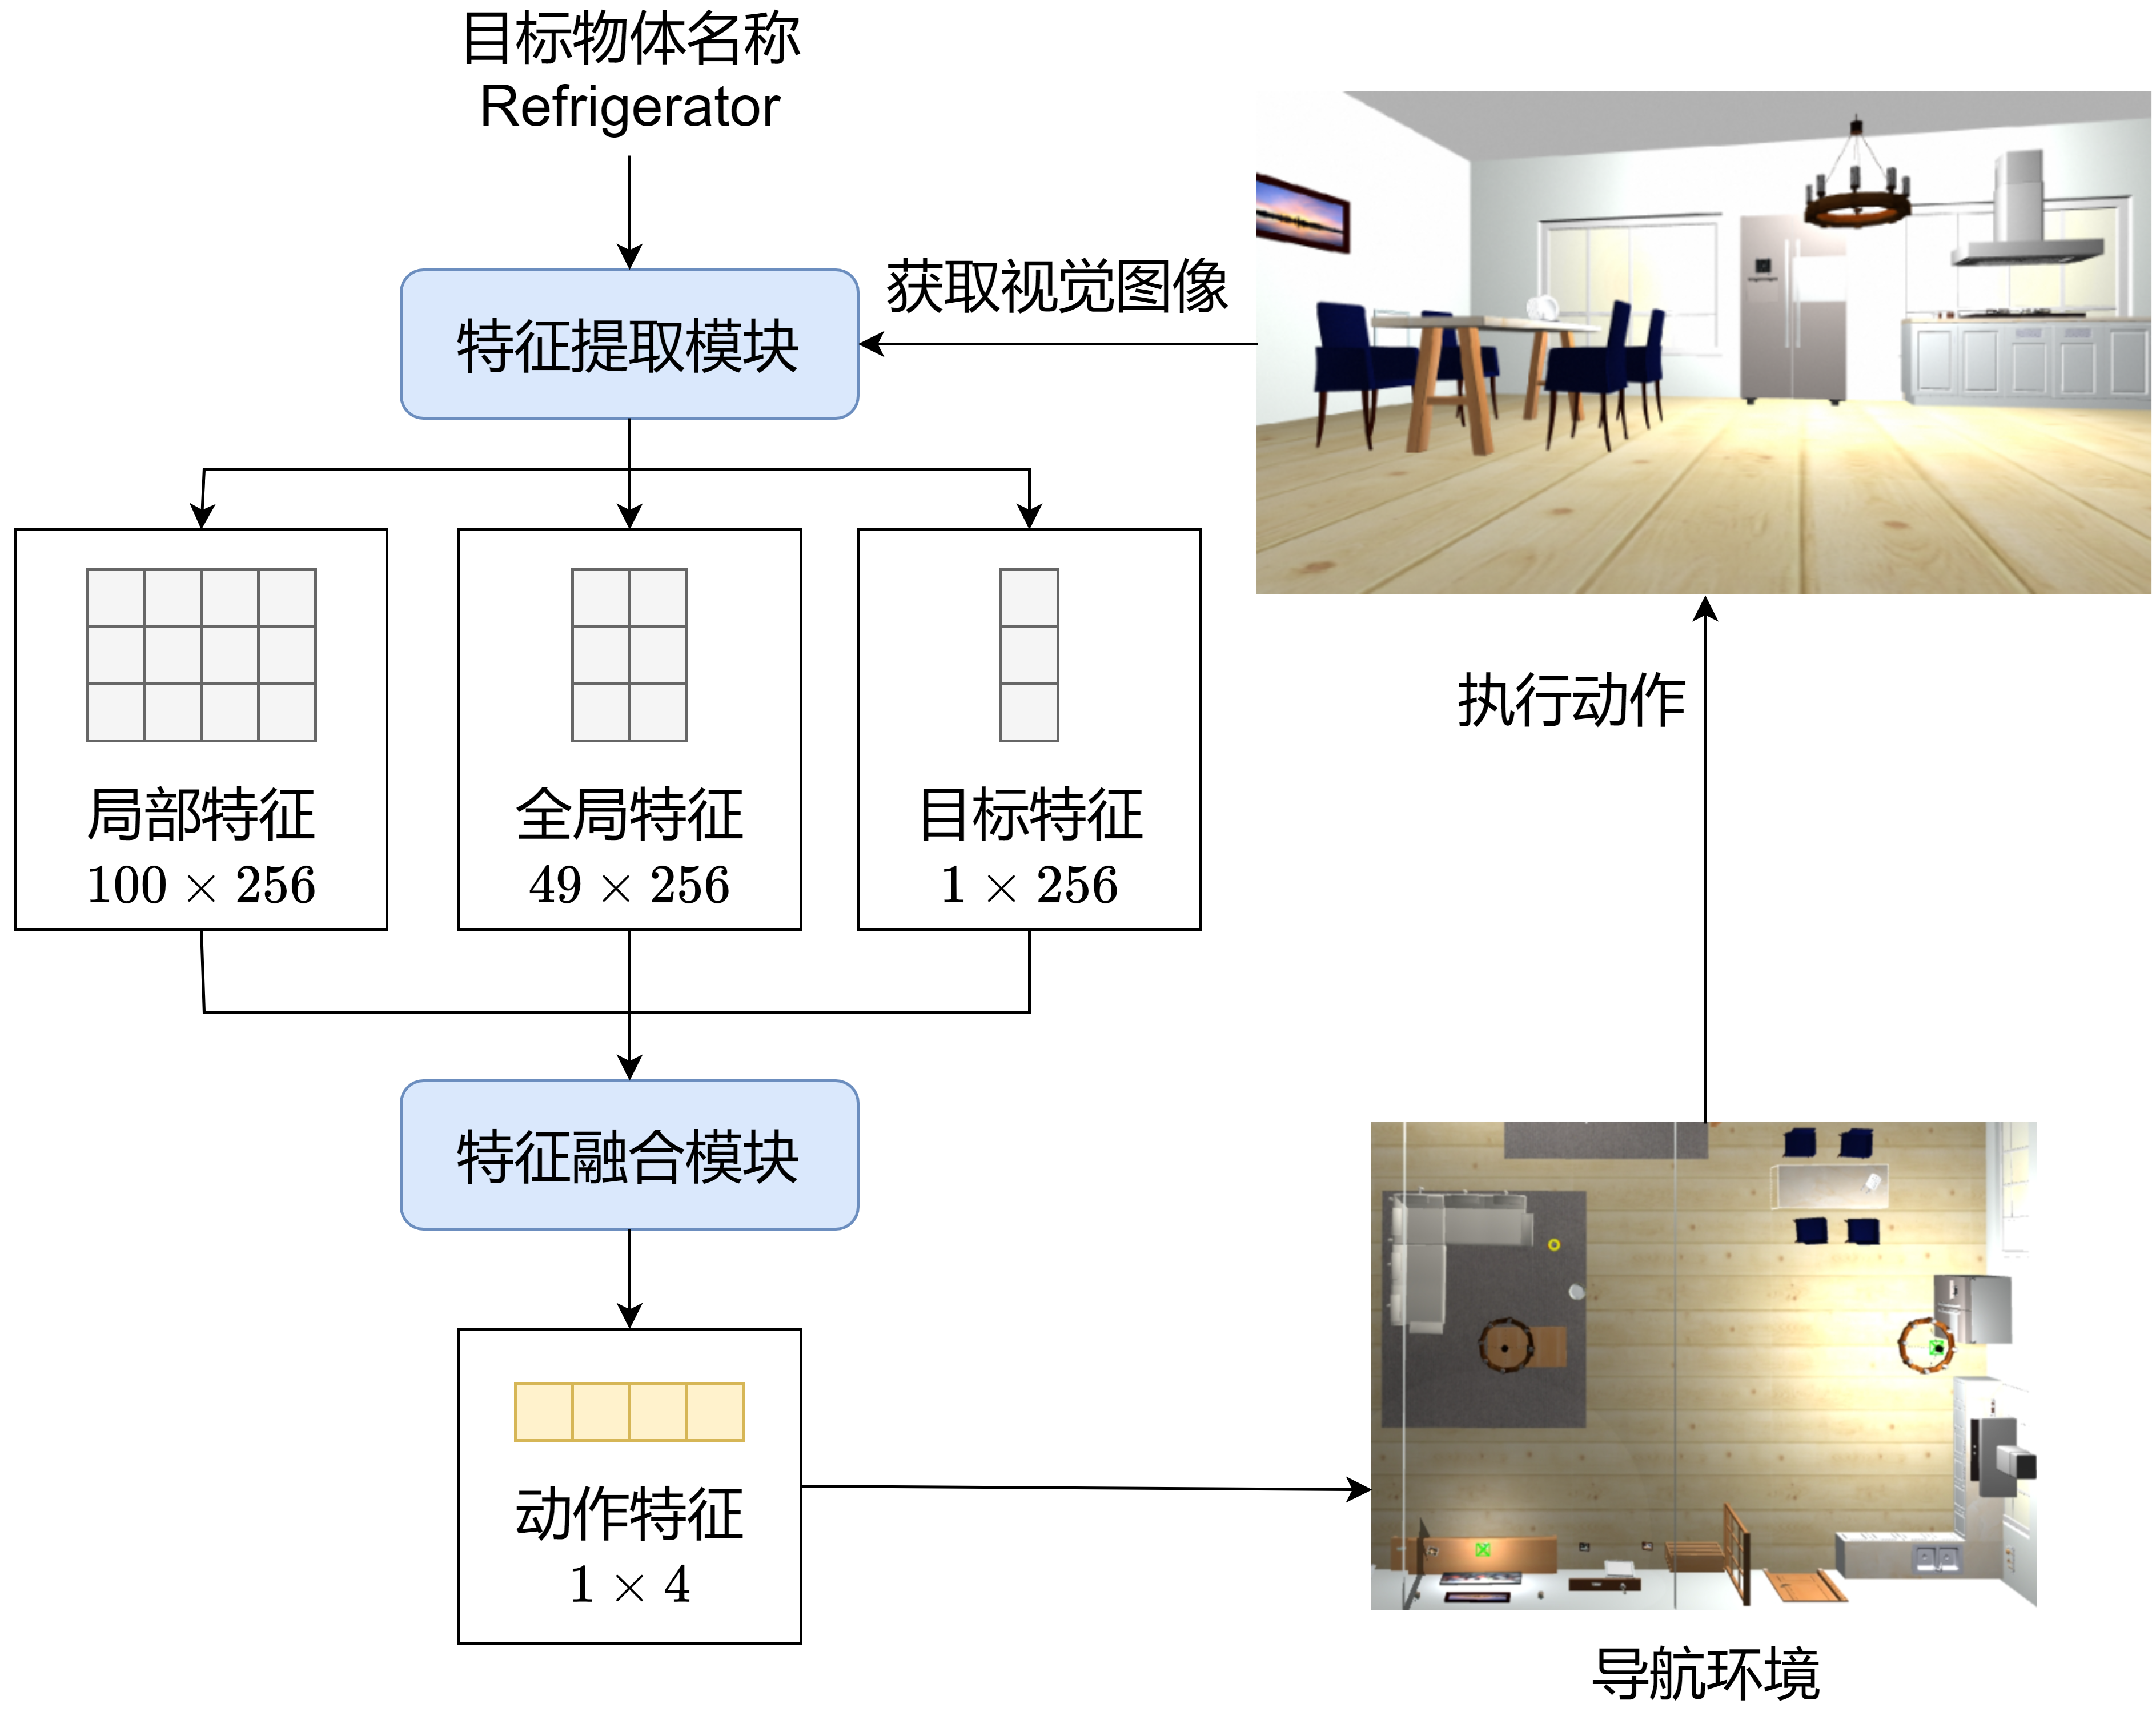
\includegraphics[scale=0.11]{Fig/提取-融合框架.png}
    \caption{\label{提取-融合框架}未知环境下的导航探索框架}
\end{figure}

上述操作过程可以用公式表示为
\begin{equation}
    {X_{{\rm{local}}}},{X_{{\rm{global}}}},{X_{{\rm{target}}}} = Extract\left( {{X_{{\rm{image}}}},{X_{{\rm{text}}}}} \right)
    \label{myeq30}
\end{equation}
\begin{equation}
    {X_{{\rm{action}}}} = Fusion\left( {{X_{{\rm{local}}}},{X_{{\rm{global}}}},{X_{{\rm{target}}}}} \right)
    \label{myeq31}
\end{equation}
其中$Extract\left( {} \right),Fusion\left( {} \right)$分别表示特征提取模块、特征融合模块,${X_{{\rm{local}}}},{X_{{\rm{global}}}},{X_{{\rm{target}}}},{X_{{\rm{image}}}},{X_{{\rm{text}}}},{X_{{\rm{action}}}}$分别表示特征提取模块中的局部特征、全局特征、目标特征、第一人称视觉图像、输入目标和特征融合模块的动作特征。



\section{特征提取模块}
在未知环境的探索导航过程中使用多层次的特征提取策略能够充分利用环境信息,使机器人在无先验知识的情况下更高效、可靠地探索并接近目标。
在未知环境下的探索导航过程中,特征提取模块主要由三个分别提取局部特征、全局特征和目标特征的不同网络组成,可以用公式表示为
\begin{equation}
{X_{{\rm{local}}}} = Concat\left( {ReLU\left( {Linear\left( {DETR\left( {{X_{{\rm{image}}}}} \right)} \right)} \right),{X_{{\rm{corelation}}}}} \right)
    \label{myeq32}
\end{equation}
\begin{equation}
{X_{{\rm{global}}}} = Flatten\left( {Conv\left( {ResNet\left( {{X_{{\rm{image}}}}} \right)} \right) + {X_{{\rm{position}}}}} \right)
    \label{myeq33}
\end{equation}
\begin{equation}
{X_{{\rm{target}}}} = Embedding\left( {{X_{{\rm{text}}}}} \right)
    \label{myeq34}
\end{equation}

经过特征提取模块处理后,表征局部环境中物体语义及其位置的局部特征、表征所处整体环境的全局特征以及表征目标物体语义的目标特征的维度均被统一成256维,处于同一个嵌入空间中。这样处理为后续特征融合模块构建出视觉观察与目标物体之间的强关联做了充分的准备,使得多种特征能够有效融合。

\subsection{提取局部特征}
局部特征的提取流程如图\ref{局部特征提取}所示。在一开始我们使用预训练的DETR网络来提取第一人称视觉RGB图像,用于表征当前视觉观察的局部信息、帮助代理认知视觉观察图像中物体代表的语义信息和位置信息,得到$100 \times 256$的局部特征,其中我们的DETR网络使用ResNet-50作为主干网络,采用六层编码器、六层解码器、八个独立注意力头和维度为2048的前馈神经网络搭建而成。然后将该特征经过全连接层Linear和ReLU激活函数以得到$100 \times 249$的局部特征,再将表征推理结果的$100 \times 7$关联特征与局部特征进行连接,得到包含环境所存在的物体语义信息、位置信息、置信度在内的$100 \times 256$的局部特征。
\begin{figure}[htbp]
    \centering
    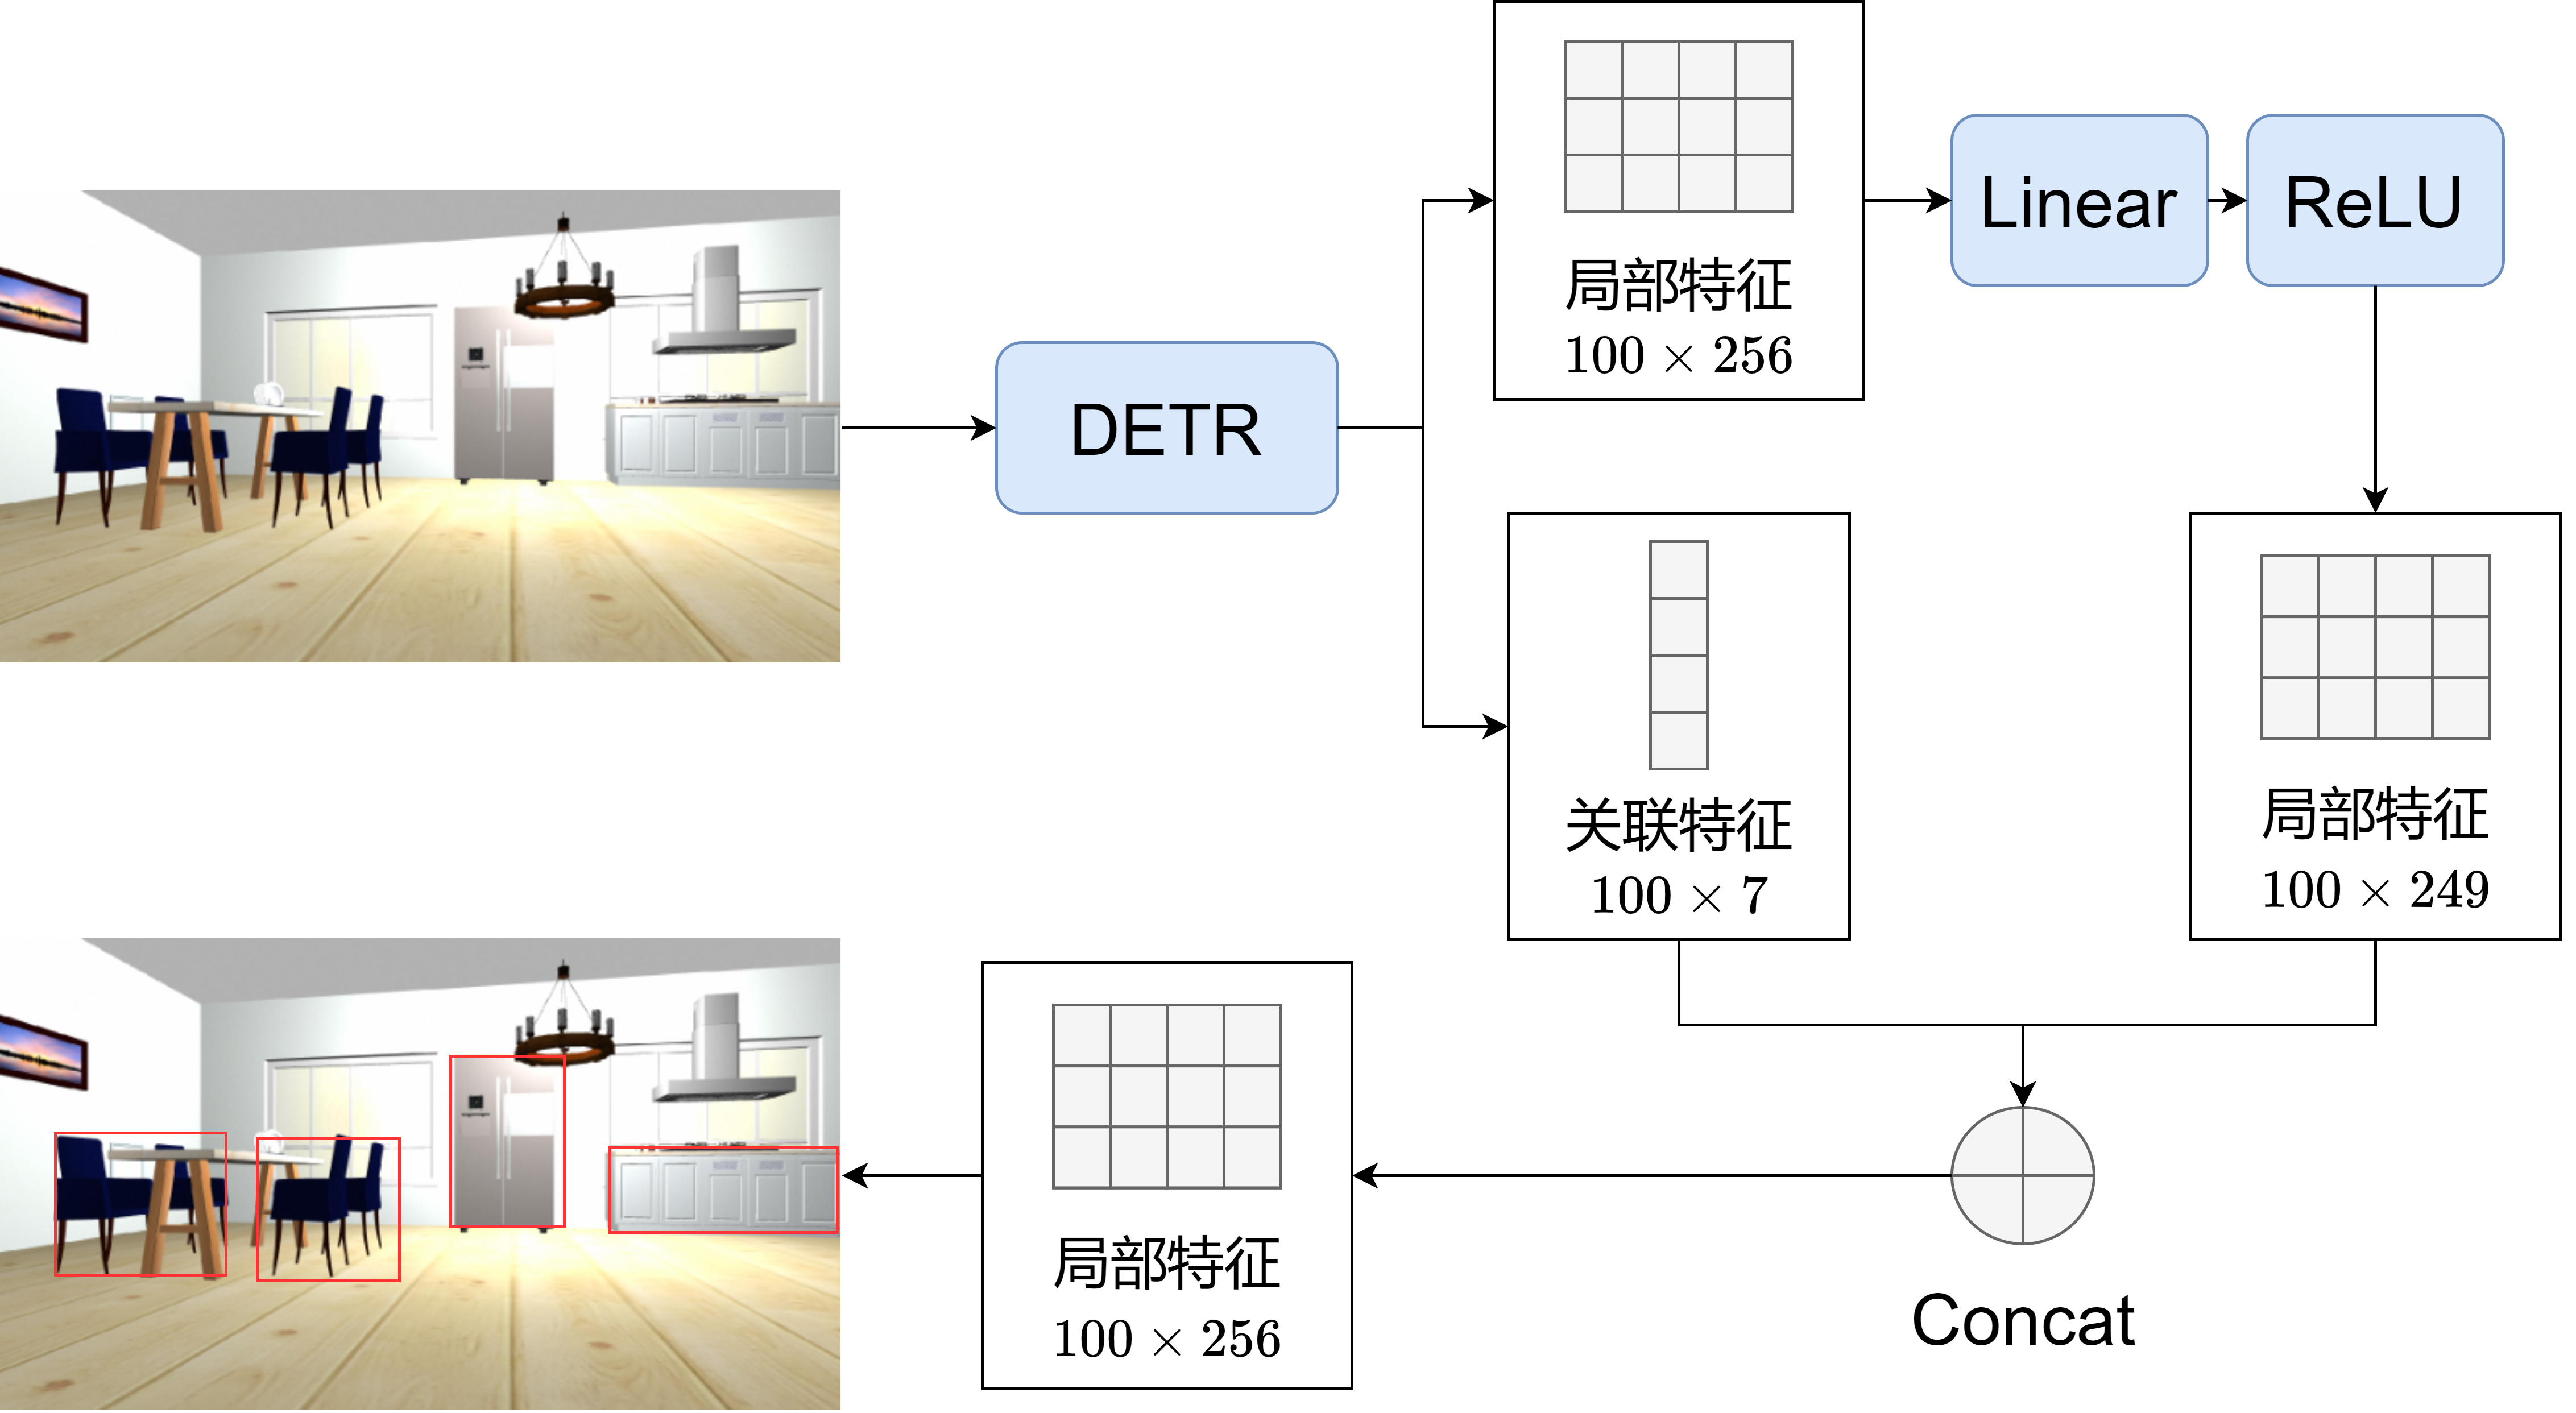
\includegraphics[scale=0.10]{Fig/局部特征提取.png}
    \caption{\label{局部特征提取}局部特征提取流程}
\end{figure}

\subsection{提取全局特征}
全局特征的提取流程如图\ref{全局特征提取}所示。我们使用ResNet18网络作为编码第一人称视觉RGB图像的网络,用于表征机器人所处当前环境的整体信息,帮助代理理解自身所处的位置信息。首先使用斯坦福大学开源的ImageNet数据集对我们搭建的ResNet18网络进行预训练,将第一人称观察视觉图像输入到该预训练的网络中再经过Conv卷积层和ReLU激活函数得到$7 \times 7 \times 256$的全局特征,再将其与通过正余弦位置编码获得的$7 \times 7 \times 256$位置特征先后进行Add操作和Flatten操作得到$49 \times 256$的全局特征。其中正余弦位置编码是一种固定、无训练参数的编码方法,它可以表示为式\ref{myeq35}\ref{myeq36},其中pos表示位置索引,i表示特征维度索引,$d_{{\rm{model}}}$表示嵌入维度即模型隐藏层维度,分母${10000^{{{2i} \mathord{\left/
 {\vphantom {{2i} {{d_{{\rm{model}}}}}}} \right.
 \kern-\nulldelimiterspace} {{d_{{\rm{model}}}}}}}}$表示用于确保不同维度的编码值在不同的频率范围内变化的缩放因子。
\begin{figure}[htbp]
    \centering
    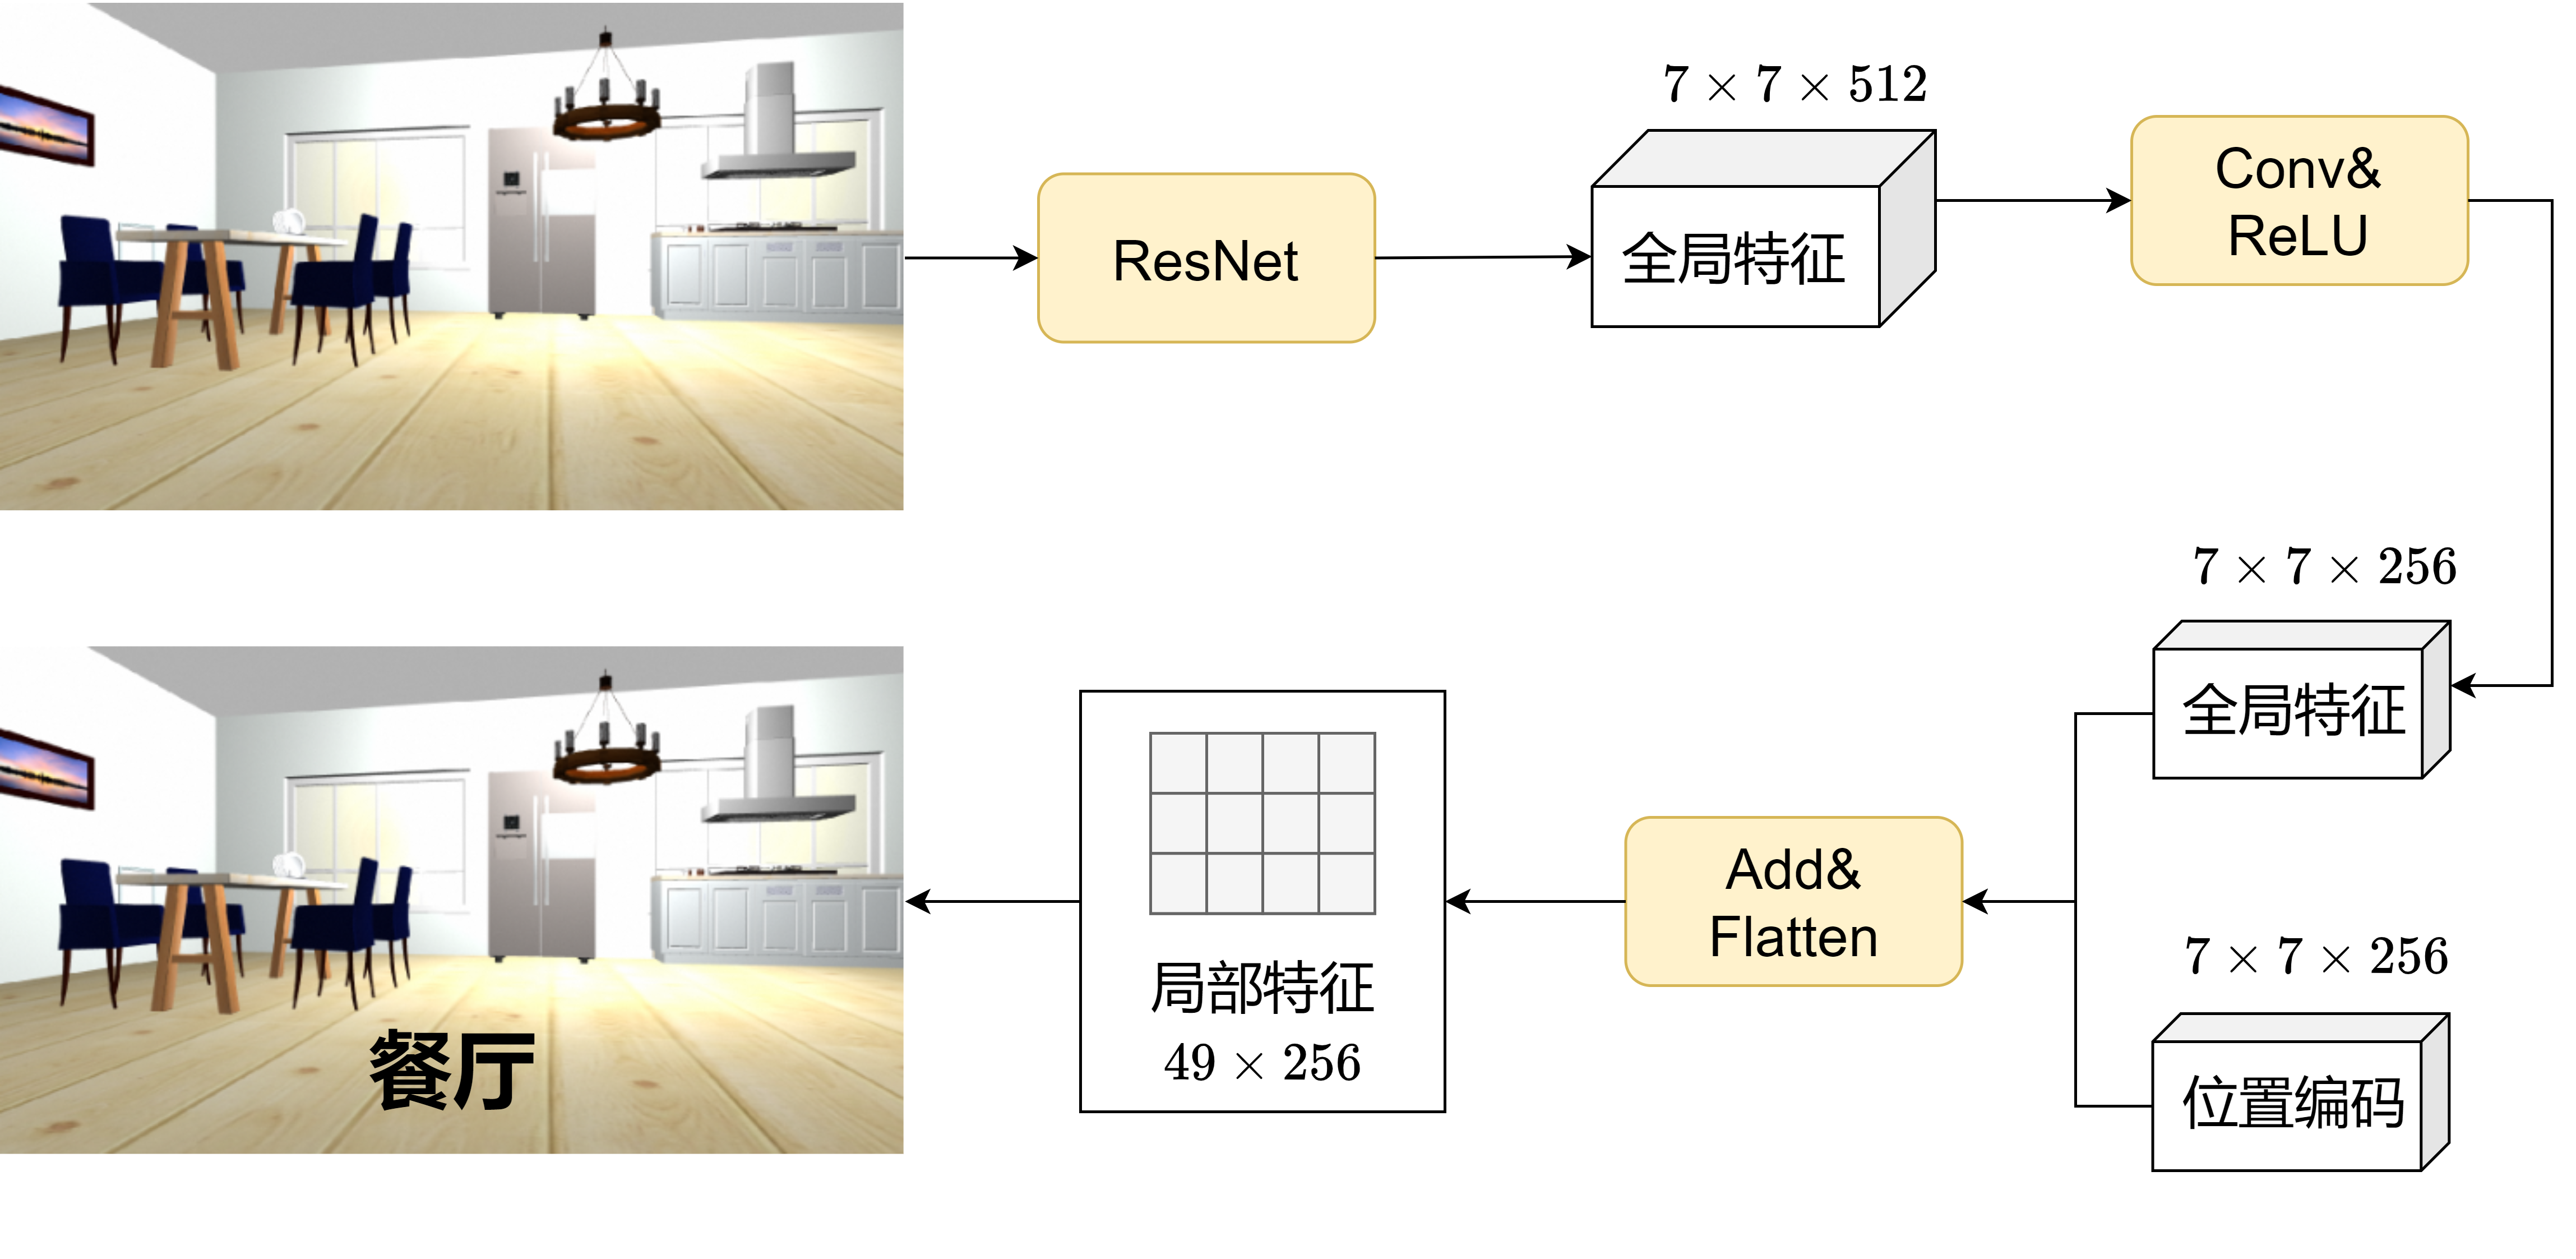
\includegraphics[scale=0.10]{Fig/全局特征提取.png}
    \caption{\label{全局特征提取}全局特征提取流程}
\end{figure}

\begin{equation}
    P{E_{\left( {pos,2i} \right)}} = \sin \left( {\frac{{pos}}{{{{10000}^{{{2i} \mathord{\left/
 {\vphantom {{2i} {{d_{{\rm{model}}}}}}} \right.
 \kern-\nulldelimiterspace} {{d_{{\rm{model}}}}}}}}}}} \right)
    \label{myeq35}
\end{equation}
\begin{equation}
    P{E_{\left( {pos,2i + 1} \right)}} = \cos \left( {\frac{{pos}}{{{{10000}^{{{2i} \mathord{\left/
 {\vphantom {{2i} {{d_{{\rm{model}}}}}}} \right.
 \kern-\nulldelimiterspace} {{d_{{\rm{model}}}}}}}}}}} \right)
    \label{myeq36}
\end{equation}

\subsection{提取目标特征}
目标特征提取流程如图\ref{目标特征提取}所示。我们首先设定词汇表大小为$V = 22$和嵌入向量维度为$D = 256$,并以此初始化嵌入矩阵$M$。随后将目标物体名称在词汇表中的索引$I$作为输入,映射到嵌入矩阵$M$以获取目标特征。在训练过程中,该目标特征会不断被优化,使语义相近的信息在嵌入空间中更加接近,从而增强特征融合模块在构建文本语义与视觉语义关联方面的能力。利用嵌入层网络对目标物体的单词进行编码可以生成用于指代目标物体语义的目标特征。在后续的特征融合过程中,可以借助注意力机制筛选出视觉观察中与目标物体相关的物体特征,从而精准确定导航的方向以快速在未知环境中找到目标。
\begin{figure}[htbp]
    \centering
    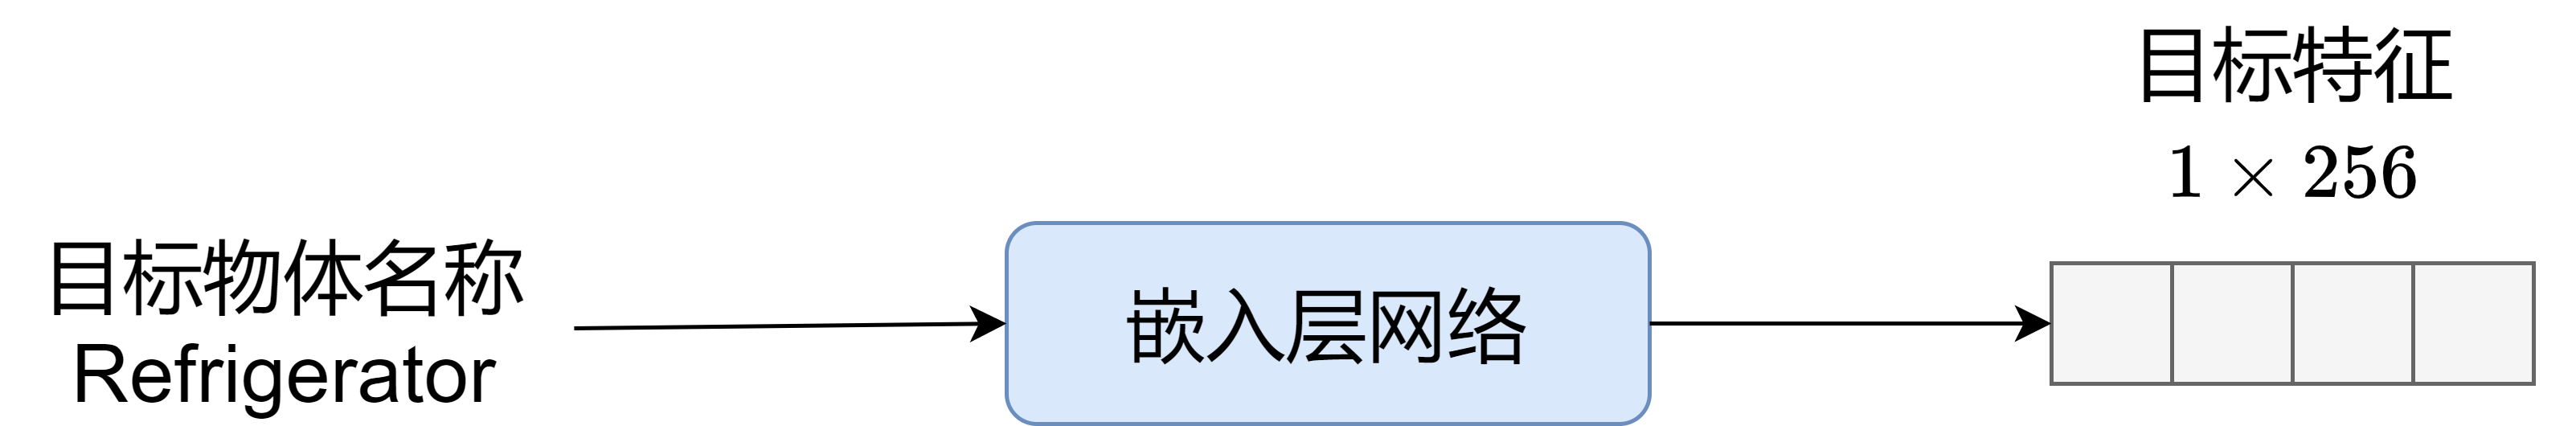
\includegraphics[scale=0.10]{Fig/目标特征提取.png}
    \caption{\label{目标特征提取}目标特征提取流程}
\end{figure}



\section{特征融合模块}
特征融合模块主要由特征融合编码器、特征融合解码器和LSTM网络构成。其中特征融合编码器主要由具有自注意力机制的Transformer encoder组成,它将特征提取模块获得的局部特征通过自注意力机制编码强化,获得能够表征表示物体与一和位置信息的强化局部特征,并将其作为键值对输入到特征融合解码器之中。特征融合解码器同样由具有多头自注意力机制的Transfomer decoder组成,它将表征目标物体语义信息和机器人所处环境位置信息的目标特征和全局特征进行强化编码,然后将作为键值对的局部特征与他们连结而成查询一同输入到网络之中,通过decoder进行融合得到环境特征和方向特征,最后,经过LSTM网络输出代理在未知环境下进行探索的离散导航动作。

我们通过观察人类在环境中寻找目标物体的过程发现,当目标物体出现在视觉观察范围内时,我们会直接按照最近的路线去靠近目标,而当目标物体未出现在观察范围内时,我们则会前往环境中存在的所有物体中与目标关联性最强的物体附近进行寻找。我们按照这样的思路去搭建特征融合网络以指导代理能够更精准的在局部未知环境中进行导航,如图\ref{未知环境导航示例图}所示,环境中存在硬纸盒、手提电脑和花盆三个物体。当需要导航到视觉观察中所发现的目标物体花盆时,代理就会根据标目标物体出现在视觉观察中的位置进行决策,执行向右前方进行移动的动作。当需要导航到视觉观察中未出现的目标物体鼠标时,代理则会先判断视觉观察中所出现的所有物体与目标物体的关联性,然后导航到手提电脑这一最可能会找到鼠标的目标旁。
\begin{figure}[htbp]
    \centering
    \includegraphics[scale=0.10]{Fig/导航示例图.png}
    \caption{\label{未知环境导航示例图}未知环境导航示例图}
\end{figure}

因此,在目标物体导航过程中代理需要从第一视角的视觉观察中提取全局特征以确定自身当前所处的位置,还需要提取局部特征以感知周围环境中物体的语义信息和位置信息。此外,代理应建立目标特征与全局特征、局部特征之间的紧密关联,从而有效引导方向特征的生成。同时,还需融合当前的全局特征与局部特征以获取环境的整体表征,并构建方向特征与环境特征相对应的序列,为后续模块提供历史经验信息,帮助LSTM网络正确地输出导航动作以指导代理在局部未知环境中进行精准高效的导航。特征融合模块的操作流程可以用如下公式表示,其中$Encoder$表示特征融合编码器,$Decoder$表示特征融合解码器。
\begin{equation}
{X_{{\rm{encoder}}}} = Encoder\left( {{X_{{\rm{local}}}}} \right)
    \label{myeq37}
\end{equation}
\begin{equation}
    {X_{{\rm{direction}}}},{X_{{\rm{environment}}}} = Decoder\left( {Concat\left( {{X_{{\rm{global}}}},{X_{{\rm{target}}}},{X_{{\rm{parameter}}}}} \right),{X_{{\rm{encoder}}}}} \right)
    \label{myeq38}
\end{equation}
\begin{equation}
    X_{{\rm{action}}}^n = Linear\left( {LSTM\left( {{X_{{\rm{direction}}}},{X_{{\rm{environment}}}},X_{{\rm{action}}}^{n - 1}} \right)} \right)
    \label{myeq39}
\end{equation}

\subsection{特征融合编码器}
特征融合模块中的编码、解码器基于Transfomer进行搭建,它的参数如表\ref{特征融合tf参数}所示,即由输入维度为256、自注意力头为8、层数为2、前馈神经网络模型的维度为512共同组成。encoder结构如图\ref{encoder}所示,我们将$100 \times 256$维的局部特征作为输入进入到encoder中的自注意力层中,经过第一次的残差连接、层归一化和前馈神经网络后经过第二次的残差连接和曾归一化,输出得到强化后的$100 \times 256$维局部特征。在encoder强化表征环境中局部物体的语义信息和未知信息的局部特征的过程之中,分为100个维度的256个序列的每一个序列都通过网络的自注意力机制与其他序列进行交互,以学习环境中物体之间的关联信息,帮助在当前视觉观察环境中未能发现目标的代理朝着与目标物体最相关联的物体方向前进,进而发现目标物体。
\begin{table}
\caption{\label{特征融合tf参数}特征融合Transfomer网络主要参数}
\centering
\small
\begin{tabular}{cccc}
    \hline
    n\_head & num\_encoder\_layers & num\_decoder\_layers & dim\_feedforward \tabularnewline 
    \hline 
    8 & 2 & 2 & 512 \tabularnewline
    \hline 
\end{tabular}
\end{table}

\begin{figure}[htbp]
    \centering
    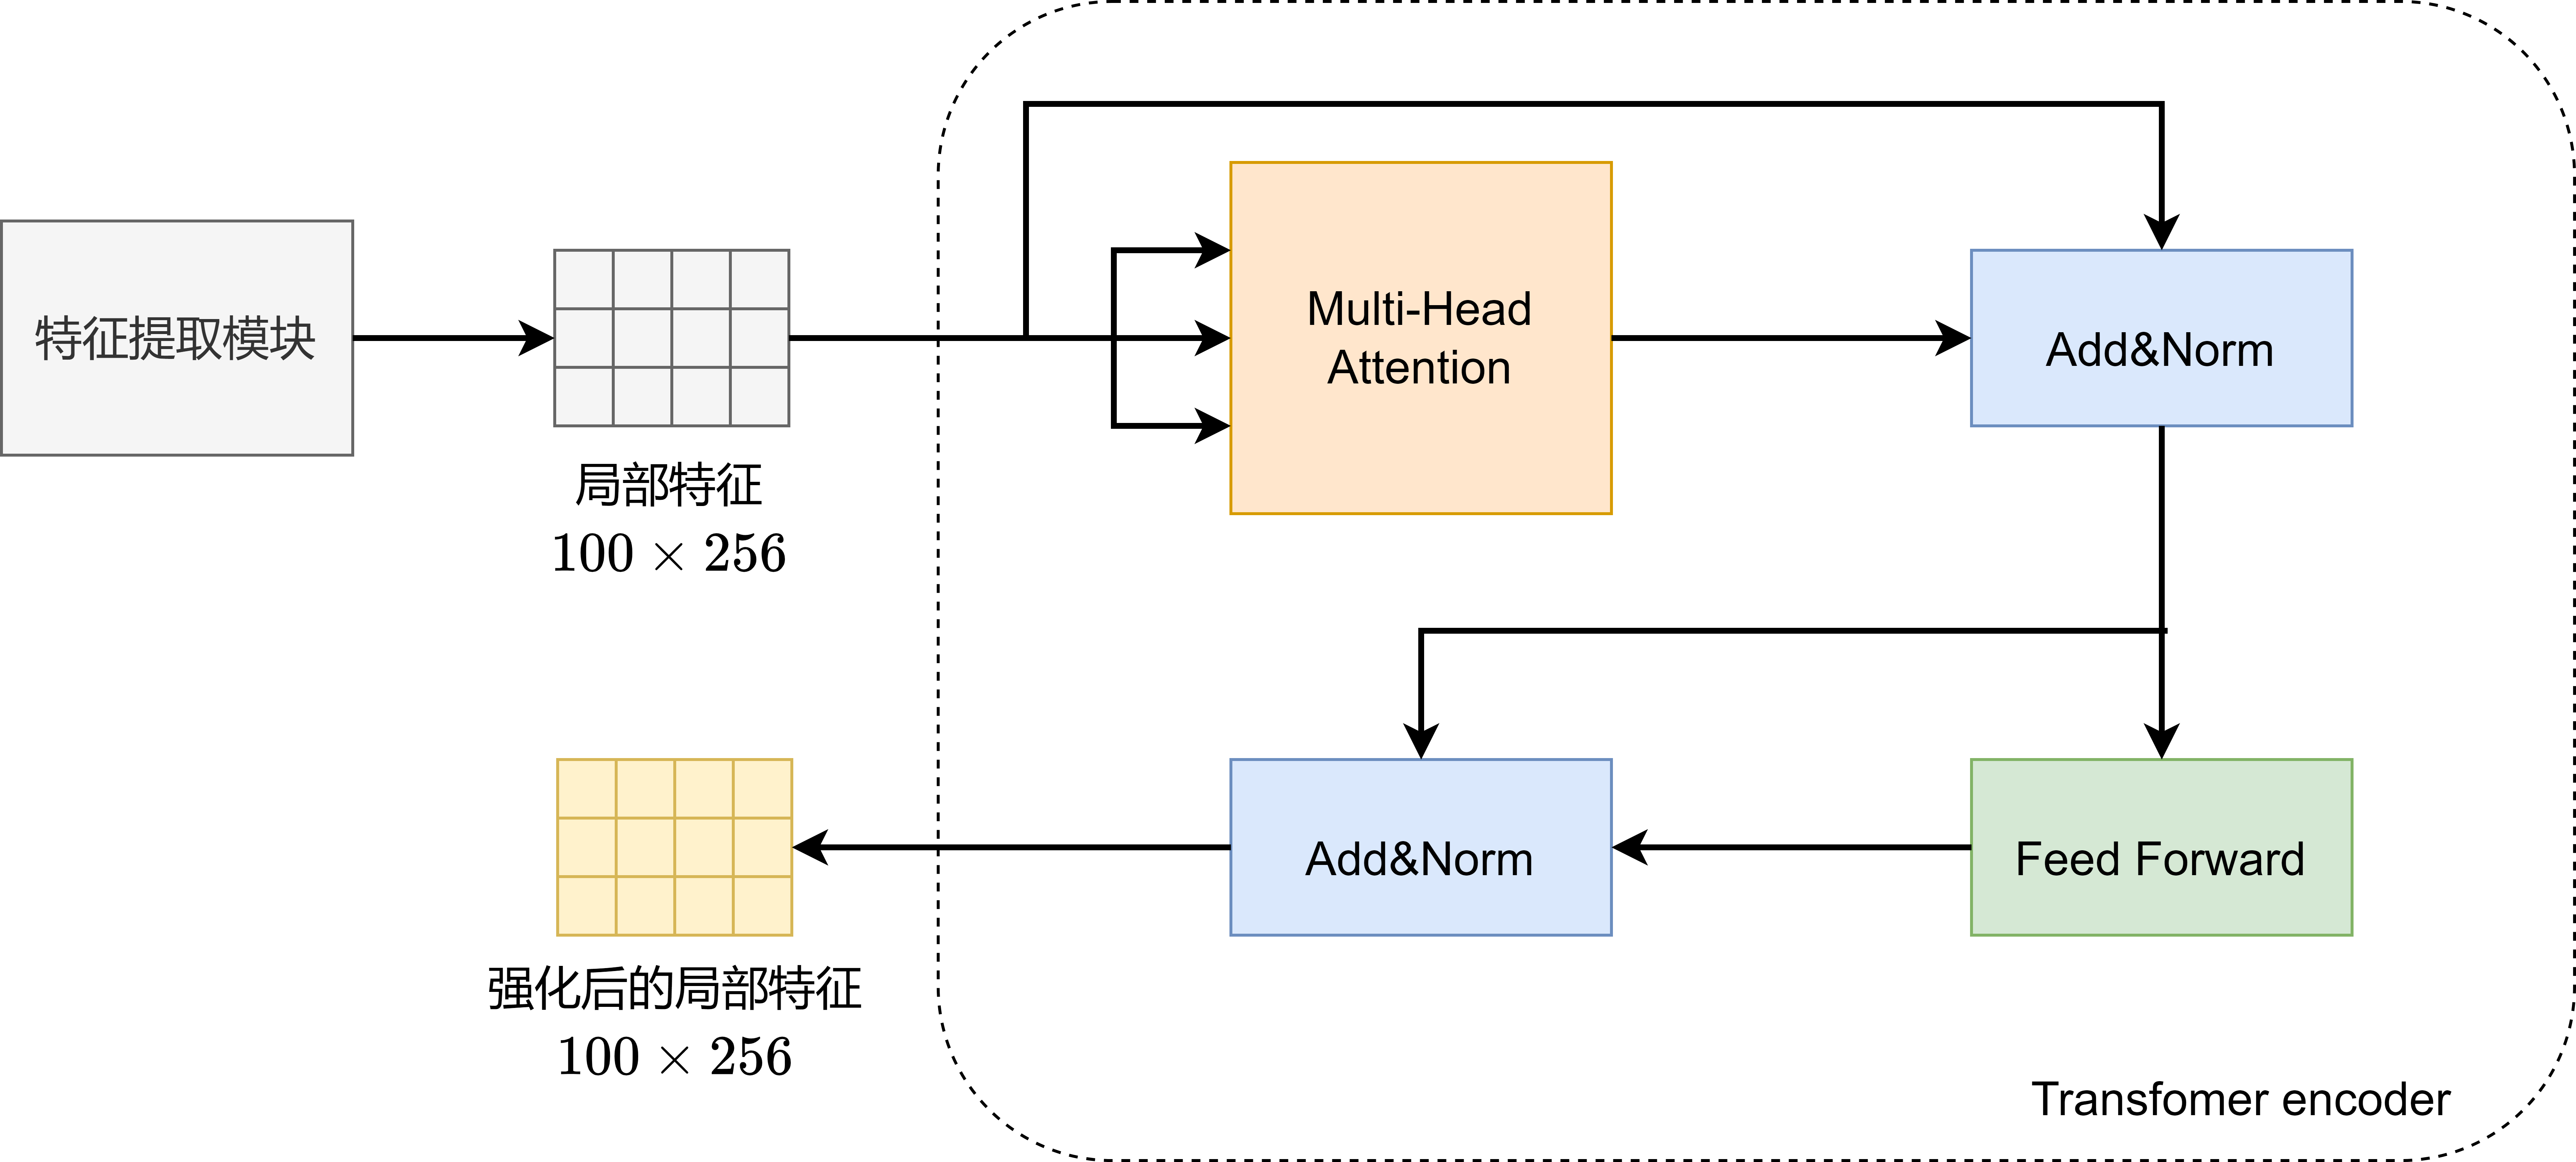
\includegraphics[scale=0.10]{Fig/encoder.png}
    \caption{\label{encoder}encoder结构图}
\end{figure}


\subsection{特征融合解码器}
特征融合的解码器decoder结构如图\ref{decoder}所示。我们将特征提取模块输出表征代理所处环境的$49 \times 256$维全局特征、表征当前导航目标的$1 \times 256$维目标特征和可学习的$1 \times 256$维目标特征进行连结,得到$51 \times 256$维的特征输入到decoder之中,在经过第一个多头自注意力层、残差连接、层归一化之后,将Transfomer encoder输出的$100 \times 256$维强化后的局部特征作为键值对、$51 \times 256$维的特征作为查询一同输入到第二个多头自注意力层之中,经过残差连接归一化层、前馈神经网络和最后一次的残差连接和层归一化后,得到$51 \times 256$维的特征,使用该特征中与$1 \times 256$维的目标特征和$1 \times 256$维的可学习的参数特征相对应位置的向量,作为表征环境中与目标相关联物体的信息,以帮助代理确定导航方向的方向特征,还有表征全局特征和局部特征共同联合的环境特征。
\begin{figure}[htbp]
    \centering
    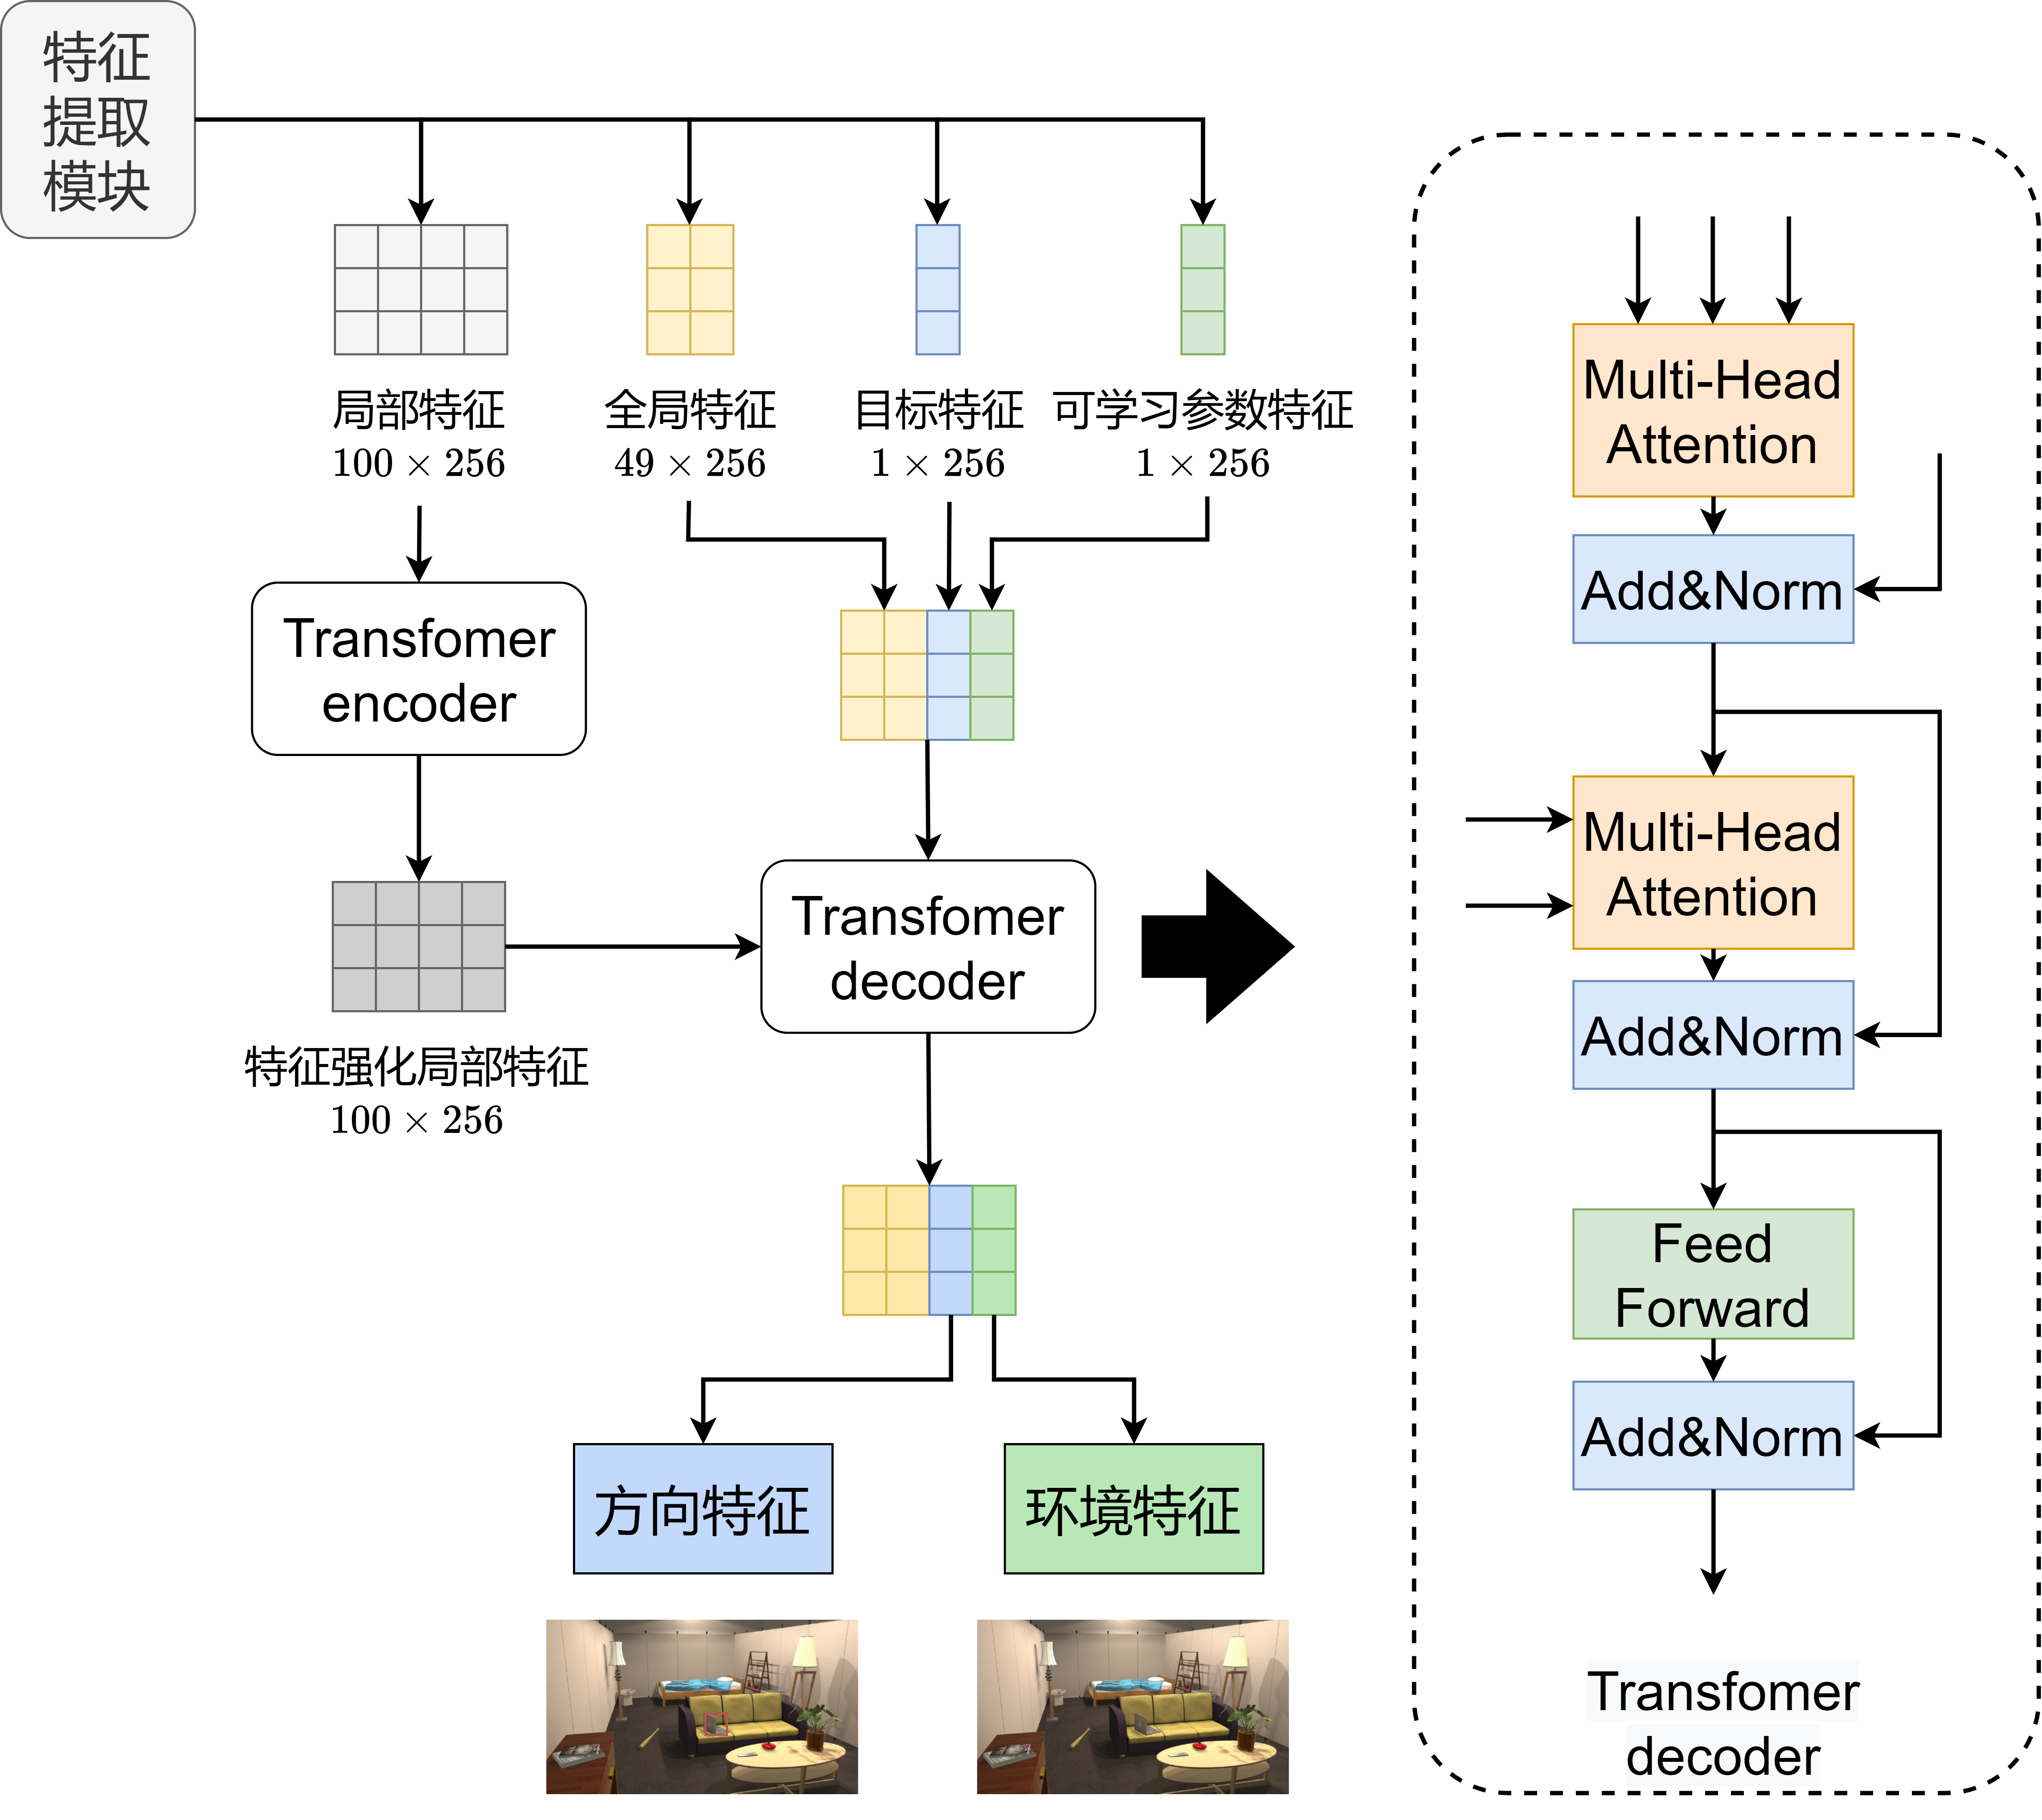
\includegraphics[scale=0.10]{Fig/decoder.png}
    \caption{\label{decoder}decoder结构图}
\end{figure}


\subsection{LSTM网络}
LSTM是一种能够有效地捕捉序列数据中的长期依赖关系的特殊循环神经网络,传统的神经网络或其他类型的RNN可能会遗忘过去的特征信息,而LSTM通过引入遗忘门、输入门和输出门从而有效地解决了这一问题,这种循环结构使得它在基于历史信息进行决策或是当任务需要依赖较长时间之前的状态时的场景中表现出色。而在机器人执行导航这种需要处理时序信息和长期依赖的任务的过程中,需要代理根据上一时刻的导航动作、方向特征和环境特征提取有用的历史信息,使用LSTM结构的网络根据以往的经验做出更精准的决策,从而达到显著提高导航系统的决策能力的目的。

通过LSTM网络输出局部未知环境下的导航动作流程如图\ref{LSTM}所示。我们将特征融合解码器输出的$1 \times 256$维方向特征、$1 \times 256$维环境特征和表示未知环境下代理所执行的$1 \times 4$维导航动作进行拼接,得到$1 \times 516$维特征向量作为双层LSTM网络的输入,最终输出$1 \times 4$维的导航动作交由运动模块所封装的导航动作执行,并且该当前时刻的导航动作在经过一个线性层后作为下一时刻的动作特征输入到LSTM网络中。
\begin{figure}[htbp]
    \centering
    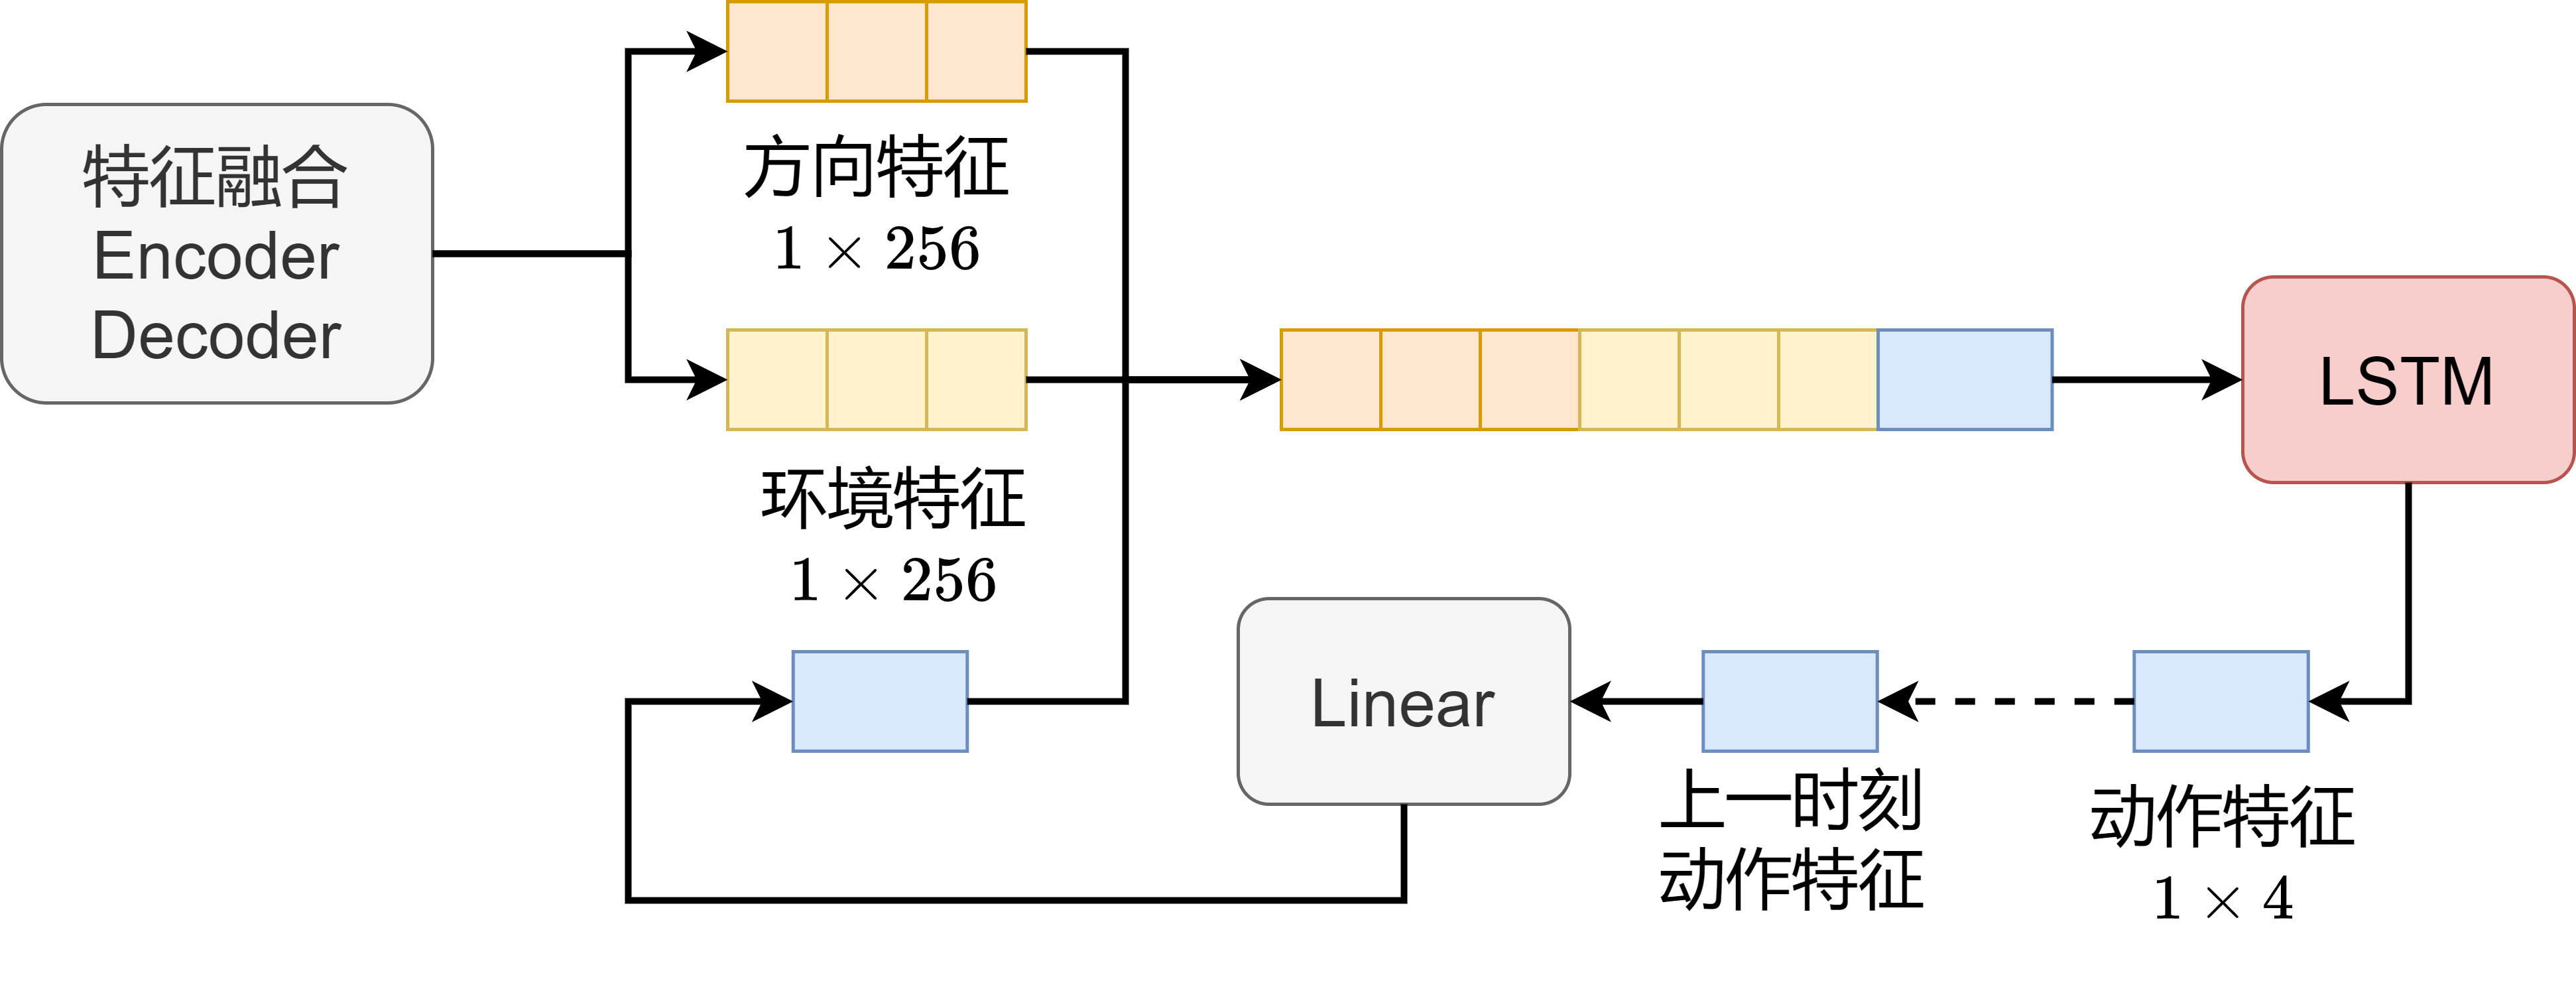
\includegraphics[scale=0.10]{Fig/LSTM.png}
    \caption{\label{LSTM}LSTM结构图}
\end{figure}


\section{运动模块}
在运动模块中,我们利用ROS节点间的通信方法来接收目标的最终位姿,借助双轮差速移动机器人的底盘移动以导航到终点。

我们的机器人采用差动模型作为其底盘的驱动方式。具体来说,机器人底盘通过调节两个轮子的转速差来控制其运动方向。当左右轮的转速相等时,机器人会沿直线行进;而当两轮的转速不同时,机器人则会围绕自身中心点进行旋转。通过合理调整两轮的转速差,机器人可以实现灵活的曲线运动和转向操作。当机器人到达目标点而需要停止动作时,可以通过完全停止轮子的转动来实现静止状态。  

具体而言,如图\ref{motion_control}所示,机器人底盘首先向电机控制板发送指令,设定左右轮的目标转速。但在实际控制过程中会受到系统误差和环境因素的影响,左右两个转轮难以精准达到设定的目标转速。为了确保机器人能够准确到达预定位置,系统引入了反馈机制,实现实时闭环的控制。电机控制板不仅需要向左右轮发送控制信号以使其接近目标转速,还需要实时采集电机编码信号。针对每个采样周期(通常为 10 毫秒),电机控制板都会累积编码脉冲的数量,并将其作为里程数据回传至底盘。底盘通过航迹推算对这些里程数据进行处理从而获取精确的里程计信息,确保机器人能够实现高精度的运动控制。
\begin{figure}[htbp]
    \centering
    \includegraphics[scale=0.07]{Fig/机器人底盘运动控制.png}
    \caption{\label{motion_control}机器人的运动控制方法}
\end{figure}

在控制移动机器人移动的过程中通常会受到地面摩擦阻力的影响,出现左右轮的实际转速和想要控制的速度不同的情况,导致移动机器人无法按照计划的轨迹进行移动,这时候就需要加入PID控制算法来调整小车的运动,使其能够精准的按照目标轨迹进行移动。

PID控制器是一种广泛使用的反馈控制系统,能够根据目标值与当前值之间的偏差来调整控制变量,从而使系统稳定地达到设定目标。具体而言,PID控制器通过调节比例、积分和微分来控制机器人的运动,确保其到达预定的位置或保持稳定的姿态,如图\ref{pid},它简单易用,适用于大多数线性控制问题,具有很好的实时性和鲁棒性。
\begin{figure}[htbp]
    \centering
    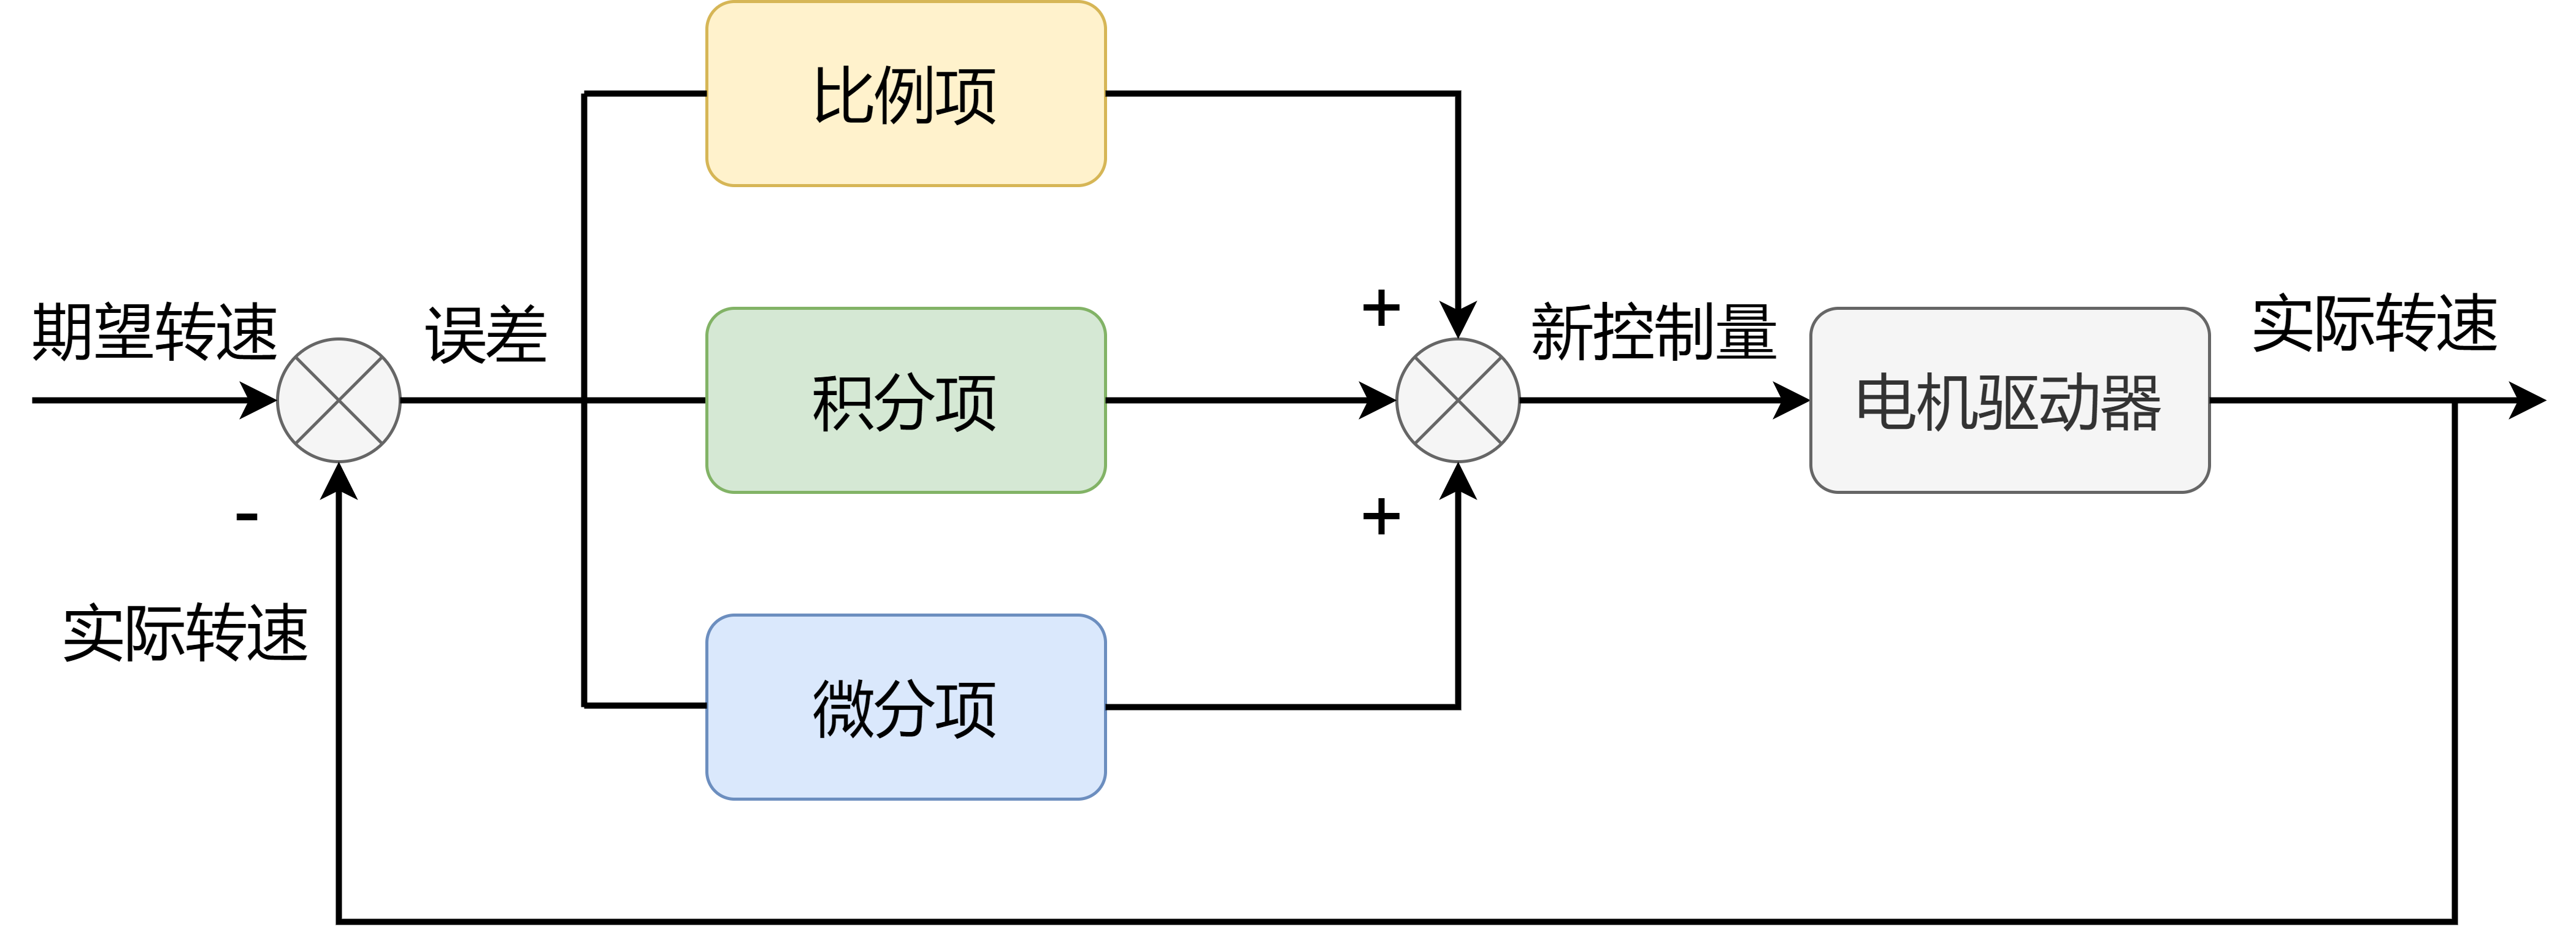
\includegraphics[scale=0.10]{Fig/pid.png}
    \caption{\label{pid}PID算法控制电机转速}
\end{figure}

比例项是PID控制器中最基础的组成部分,它直接根据期望值与实际值之间的偏差来进行调整,如式\ref{myeq17},其中$P$表示比例控制输出,${K_p}$表示比例增益,即在误差变化时控制器输出的变化幅度,$e\left( t \right)$表示当前时刻的误差,当误差越大时,比例项的输出也就越大,以帮助系统更快速的接近目标值。
\begin{equation}
    P = {K_p} \cdot e\left( t \right)
    \label{myeq17}
\end{equation}

积分项是PID控制器中的第二个组成部分。积分项的目的是消除系统在长时间运行中可能出现的静态误差,确保系统达到并保持在期望的目标位置,如式\ref{myeq18},其中$I$表示积分控制输出,${K_i}$表示积分增益,能够决定积分项对控制输出的影响程度,${e\left( t \right)}$表示误差。当系统的输出长期无法达到设定的目标时,积分项就会逐渐地累积来弥补系统长期积累的偏差,一直到该误差消除。
\begin{equation}
    I = {K_i} \cdot \int_0^t {e\left( t \right)dt} 
    \label{myeq18}
\end{equation}

当积分增益过大时会导致系统响应过度,引发系统的超调和震荡,这时候就需要通过微分项来预测误差的变化趋势以减少系统发生超调和震荡的可能。与前面介绍的两者不同,微分项主要关注的是误差变化的速度而非当前的误差值,如式\ref{myeq19},其中$D$表示微分控制输出,${K_d}$表示决定了微分项对控制输出的影响程度的微分增益,$\frac{d}{{dt}}e\left( t \right)$表示用来预测未来误差变化趋势的误差变化速率。通过微分项的预测误差和提前调整,系统能够避免震荡和过调现象的发生,让系统更加平稳的响应。
\begin{equation}
    D = {K_d} \cdot \frac{d}{{dt}}e\left( t \right)
    \label{myeq19}
\end{equation}
通常情况下积分项、比例项和微分项会一起使用,即通过比例项消除实时误差,利用积分项来消除长期累计的误差,而微分项则通过对误差变化率的敏感度调整来预测误差的变化趋势,减少系统发生超调和震荡的概率,三者相辅相成一同构成一个完整的PID控制器,使其能够更精准、更平稳地调节系统响应。

在移动机器人根据多特征融合网络的输出进行局部范围内的探索以期找到目标物体时,我们需要计算出每一时刻的里程计数据,并将其与订阅获取的实时里程计数据进行比较,从而计算出当前已经移动的距离,达到让机器人准确地进行移动的目的。具体来说里程计包括位姿(位置和方向角)和运动速度(线速度与角速度)两个重要的信息,它的计算过程如图\ref{motion_calculate}所示。在整个机器人运动的过程当中,假设用${p_i}$来表示在时刻$i$的位姿,图中的${p_1},{p_2}, \ldots ,{p_n}$则代表机器人的整个运动过程中的轨迹。在很短的时间内,机器人从${p_1}$运动到${p_2}$,那么我们就可以根据机器人当前的位姿${p_1}$及其左右轮的速度${V_{left}}$和${V_{right}}$,通过微积分的方法来推算机器人下一个时间步${p_2}$处的线速度、角速度及其位姿,从而计算获得完整的里程计数据。
\begin{figure}[htbp]
    \centering
    \includegraphics[scale=0.05]{Fig/移动控制.png}
    \caption{\label{motion_calculate}里程计计算}
\end{figure}

机器人自身的坐标系用于描述相对位置信息,而世界坐标系用于刻画机器人的全局状态,且世界坐标系与机器人自身的坐标系在初始时刻重合。在任意时刻$t$,机器人的位姿可以表示为${P_t} = \left( {{x_t},{y_t},{\theta _t}} \right)$,其中$\left( {{x_t},{y_t}} \right)$表示机器人在世界坐标系下的位置,${{\theta _t}}$表示朝向角。我们的移动机器人采用双轮差速模型进行驱动,其运动可以近似视为围绕某一瞬时旋转中心,以半径r沿圆弧轨迹运动。已知左右轮的速度${V_{left}}$、${V_{right}}$及两轮间距$l$,可以通过式\eqref{myeq20}、\eqref{myeq21}和\eqref{myeq22}来计算机器人在$t$时刻的线速度$v$、角速度$\omega $以及旋转半径$r$
\begin{equation}
    v = \frac{{{v_{left}} + {v_{right}}}}{2}
    \label{myeq20}
\end{equation}
\begin{equation}
    \omega  = \frac{{{v_{right}} - {v_{left}}}}{l}\left( {{{rad} \mathord{\left/
 {\vphantom {{rad} s}} \right.
 \kern-\nulldelimiterspace} s}} \right)
    \label{myeq21}
\end{equation}
\begin{equation}
    r = \frac{v}{\omega } = \frac{l}{2} \cdot \frac{{{v_{right}} + {v_{left}}}}{{{v_{right}} - {v_{left}}}}
    \label{myeq22}
\end{equation}

在实际计算中,我们采用速度积分法推算机器人在时刻的位姿。设在t-1时刻移动机器人的位姿为${P_t} = \left( {{x_{t - 1}},{y_{t - 1}},{\theta _{t - 1}}} \right)$,当机器人在极短的$\Delta t$时间内进行运动时可以视为是匀速运动,这是可以通过如下递推式\eqref{myeq23}、\eqref{myeq24}和\eqref{myeq25}计算出结果。
\begin{equation}
{\theta _t} = {\theta _{t - 1}} + \omega  * \Delta t
    \label{myeq23}
\end{equation}
\begin{equation}
    {x_t} = {x_{t - 1}} + r * \left( {\sin {\theta _t} - \sin {\theta _{t - 1}}} \right)
    \label{myeq24}
\end{equation}
\begin{equation}
{y_t} = {y_{t - 1}} - r * \left( {\cos {\theta _t} - \cos {\theta _{t - 1}}} \right)
    \label{myeq25}
\end{equation}
该方法能够高效、准确地计算机器人每个时刻的位姿,并依次累积得到完整的运动轨迹,为导航和路径规划提供精确的里程计数据支持。在具体的实现中我们将上述计算流程进行封装,针对每一种离散动作指令都编写对应的函数用于机器人在未知环境中进行探索。

\section{图像点云融合模块}
在未知环境的目标物体导航任务中,要求代理要具备识别出环境中存在着的目标物体的功能。多线激光雷达具备高精度的深度测量能力,能够提供目标的距离感知信息和三维结构,但点云数据会随着距离的变大而逐渐变得稀疏,在追踪远距离目标时效果有限。单目相机则具有高分辨率的视觉信息,能够捕捉目标的纹理、颜色和边缘特征等认知信息,但缺乏直接的深度感知能力,且容易受到光照条件等环境因素的影响。相比于使用单一传感器进行检测,通过多线激光和单目相机的联合检测方法能够有效降低误检和漏检率,在各种应用场景中展现出显著的优势。首先图像点云融合方法能够显著提升代理对远距离目标检测能力,即使在单目相机难以判别目标的远距离区域,依旧可以通过多线激光雷达来获取准确的深度信息。并且目前的视觉言语导航方法大多仅依赖于网络模型输出的动作进行决策,使用导航至目标3米内即算完成导航任务这一笼统指标并不利于后续利用机械臂执行的下游任务的执行,这就需要多线激光提供的准确距离信息来辅助代理进行导航,以完成导航至目标半米内的任务。

局部路径规划方法中的图像点云融合模块使用了第二章所介绍的YOLOV10目标检测网络、优化后的欧式点云聚类算法和多线激光单目相机联合标定方法。多线激光获取的点云在经过点云聚类之后通过外参矩阵重投影到目标检测二维图像上,并且使用IoU重叠度(Intersection over Union)来判断目标检测框中的目标物体与点云聚类结果是否匹配,当点云聚类结果与目标检测框不匹配时就会被舍弃,当结果匹配时就会被纳入结果集,并将出所选定的区域框中所有点云的均值作为该目标的距离,用以发布最终导航目标点完成完整的导航。

IoU具有非负性、不可分辨的同一性、对称性和尺度不变这类属性,这使得通过这个方法来判断两个任意形状A和B之间的相似性与它们的空间尺度无关,所以它被广泛用作计算机视觉中许多任务的评估指标,如像素级图像分割、2D和3D对象检测等。
因此,本文使用IoU度量法来衡量有限的点云聚类算法结果和目标检测算法结果之间的相似性。具体来说针对两个有限样本集合$A$和$B$,他们之间的IoU被定义为他们的交集除以他们之间的并集,如式\ref{myeq26}。
\begin{equation}
    {\rm{IoU}}\left( {A,B} \right) = \frac{{A \cap B}}{{A \cup B}} = \frac{{A \cap B}}{{\left| A \right| + \left| B \right| - A \cap B}}
    \label{myeq26}
\end{equation}

根据点云聚类和目标检测的结果可以获得两个不同的预选框,将他们通过预选框匹配算法计算他们之间的IoU度量,如算法\ref{algorithm3}。当预选框之间的IoU小于0.5时,认为它们属于独立不同的检测对象;当IoU介于0.4到0.8之间时,则将重叠区域作为最终目标区域;当IoU介于0.8到1之间时,两个检测框基本重合,此时认为两者的边界都是有效的,将使用边界框的扩展区域作为最终的融合结果框,如图\ref{iou}。
\begin{algorithm}[!h]
    \caption{IoU度量算法}
    \label{algorithm3}
    \renewcommand{\algorithmicrequire}{\textbf{Input:}}
    \renewcommand{\algorithmicensure}{\textbf{Output:}}
    \renewcommand{\algorithmiccomment}[1]{\hfill $\triangleright$ #1}
    \begin{algorithmic}[1]
        \REQUIRE 检测框的四个角坐标:
        $\begin{array}{l}
            {A_1}\left( {{x_1},{y_1}} \right),{B_1}\left( {{x_2},{y_1}} \right),{C_1}\left( {{x_2},{y_2}} \right),{D_1}\left( {{x_1},{y_2}} \right)\\
            {A_1}\left( {{{x'}_1},{{y'}_1}} \right),{B_1}\left( {{{x'}_2},{{y'}_1}} \right),{C_1}\left( {{{x'}_2},{{y'}_2}} \right),{D_1}\left( {{{x'}_1},{{y'}_2}} \right)\\
            {x_1} \le {x_2},{y_2} \le {y_1},{{x'}_1} \le {{x'}_2},{{y'}_2} \le {{y'}_1}
            \end{array}$  %%input
        \ENSURE 两个预选框之间的IoU结果   %%output
        \STATE  The area of ${{\rm{B}}_{{\rm{c }}}}$:${\rm{Are}}{{\rm{a}}_{\rm{c}}} = ({x_2} - {x_1}) \times ({y_1} - {y_2})$
        \STATE  The area of ${{\rm{B}}_{{\rm{d }}}}$:${\rm{Are}}{{\rm{a}}_{\rm{d}}} = ({{x'}_2} - {{x'}_1}) \times ({{y'}_1} - {{y'}_2})$
		\STATE  The area of overlap:\\
        ${\rm{Are}}{{\rm{a}}_{{\rm{overlap}}}} = (\max ({x_2} - {{x'}_2}) - \min ({x_1},{{x'}_1})) \times (\max ({y_1} - {{y'}_1}) - \min ({y_2},{{y'}_2}))$
		\STATE  ${\rm{IoU}} = {\rm{Are}}{{\rm{a}}_{{\rm{overlap}}}}/({\rm{Are}}{{\rm{a}}_c} + {\rm{Are}}{{\rm{a}}_d} - {\rm{Are}}{{\rm{a}}_{{\rm{overlap}}}})$
    \end{algorithmic}
\end{algorithm}
\begin{figure}[htbp]
    \centering
    \includegraphics[scale=0.11]{Fig/iou.png}
    \caption{\label{iou}预选框选择策略}
\end{figure}

在经过预选框选择策略之后获得的最终边界框将用于测定目标在机器人坐标系下的位姿,如图\ref{target_pose}。通过最终边界框的中点$\left( {{u_{mid}},{v_{mid}}} \right)$和单目相机的水平视域、垂直视域,可以分别计算出目标物体与机器人$x$轴正方向的水平夹角$\phi $、目标物体与机器人$y$轴正方向的水平夹角$\varphi $。然后将投影在最终边界框中的点云距离进行均值相加以获得机器人与目标之间的距离$D$,根据$\phi $、$\varphi $和$D$可以计算出机器人坐标系下目标的位姿。
\begin{figure}[htbp]
    \centering
    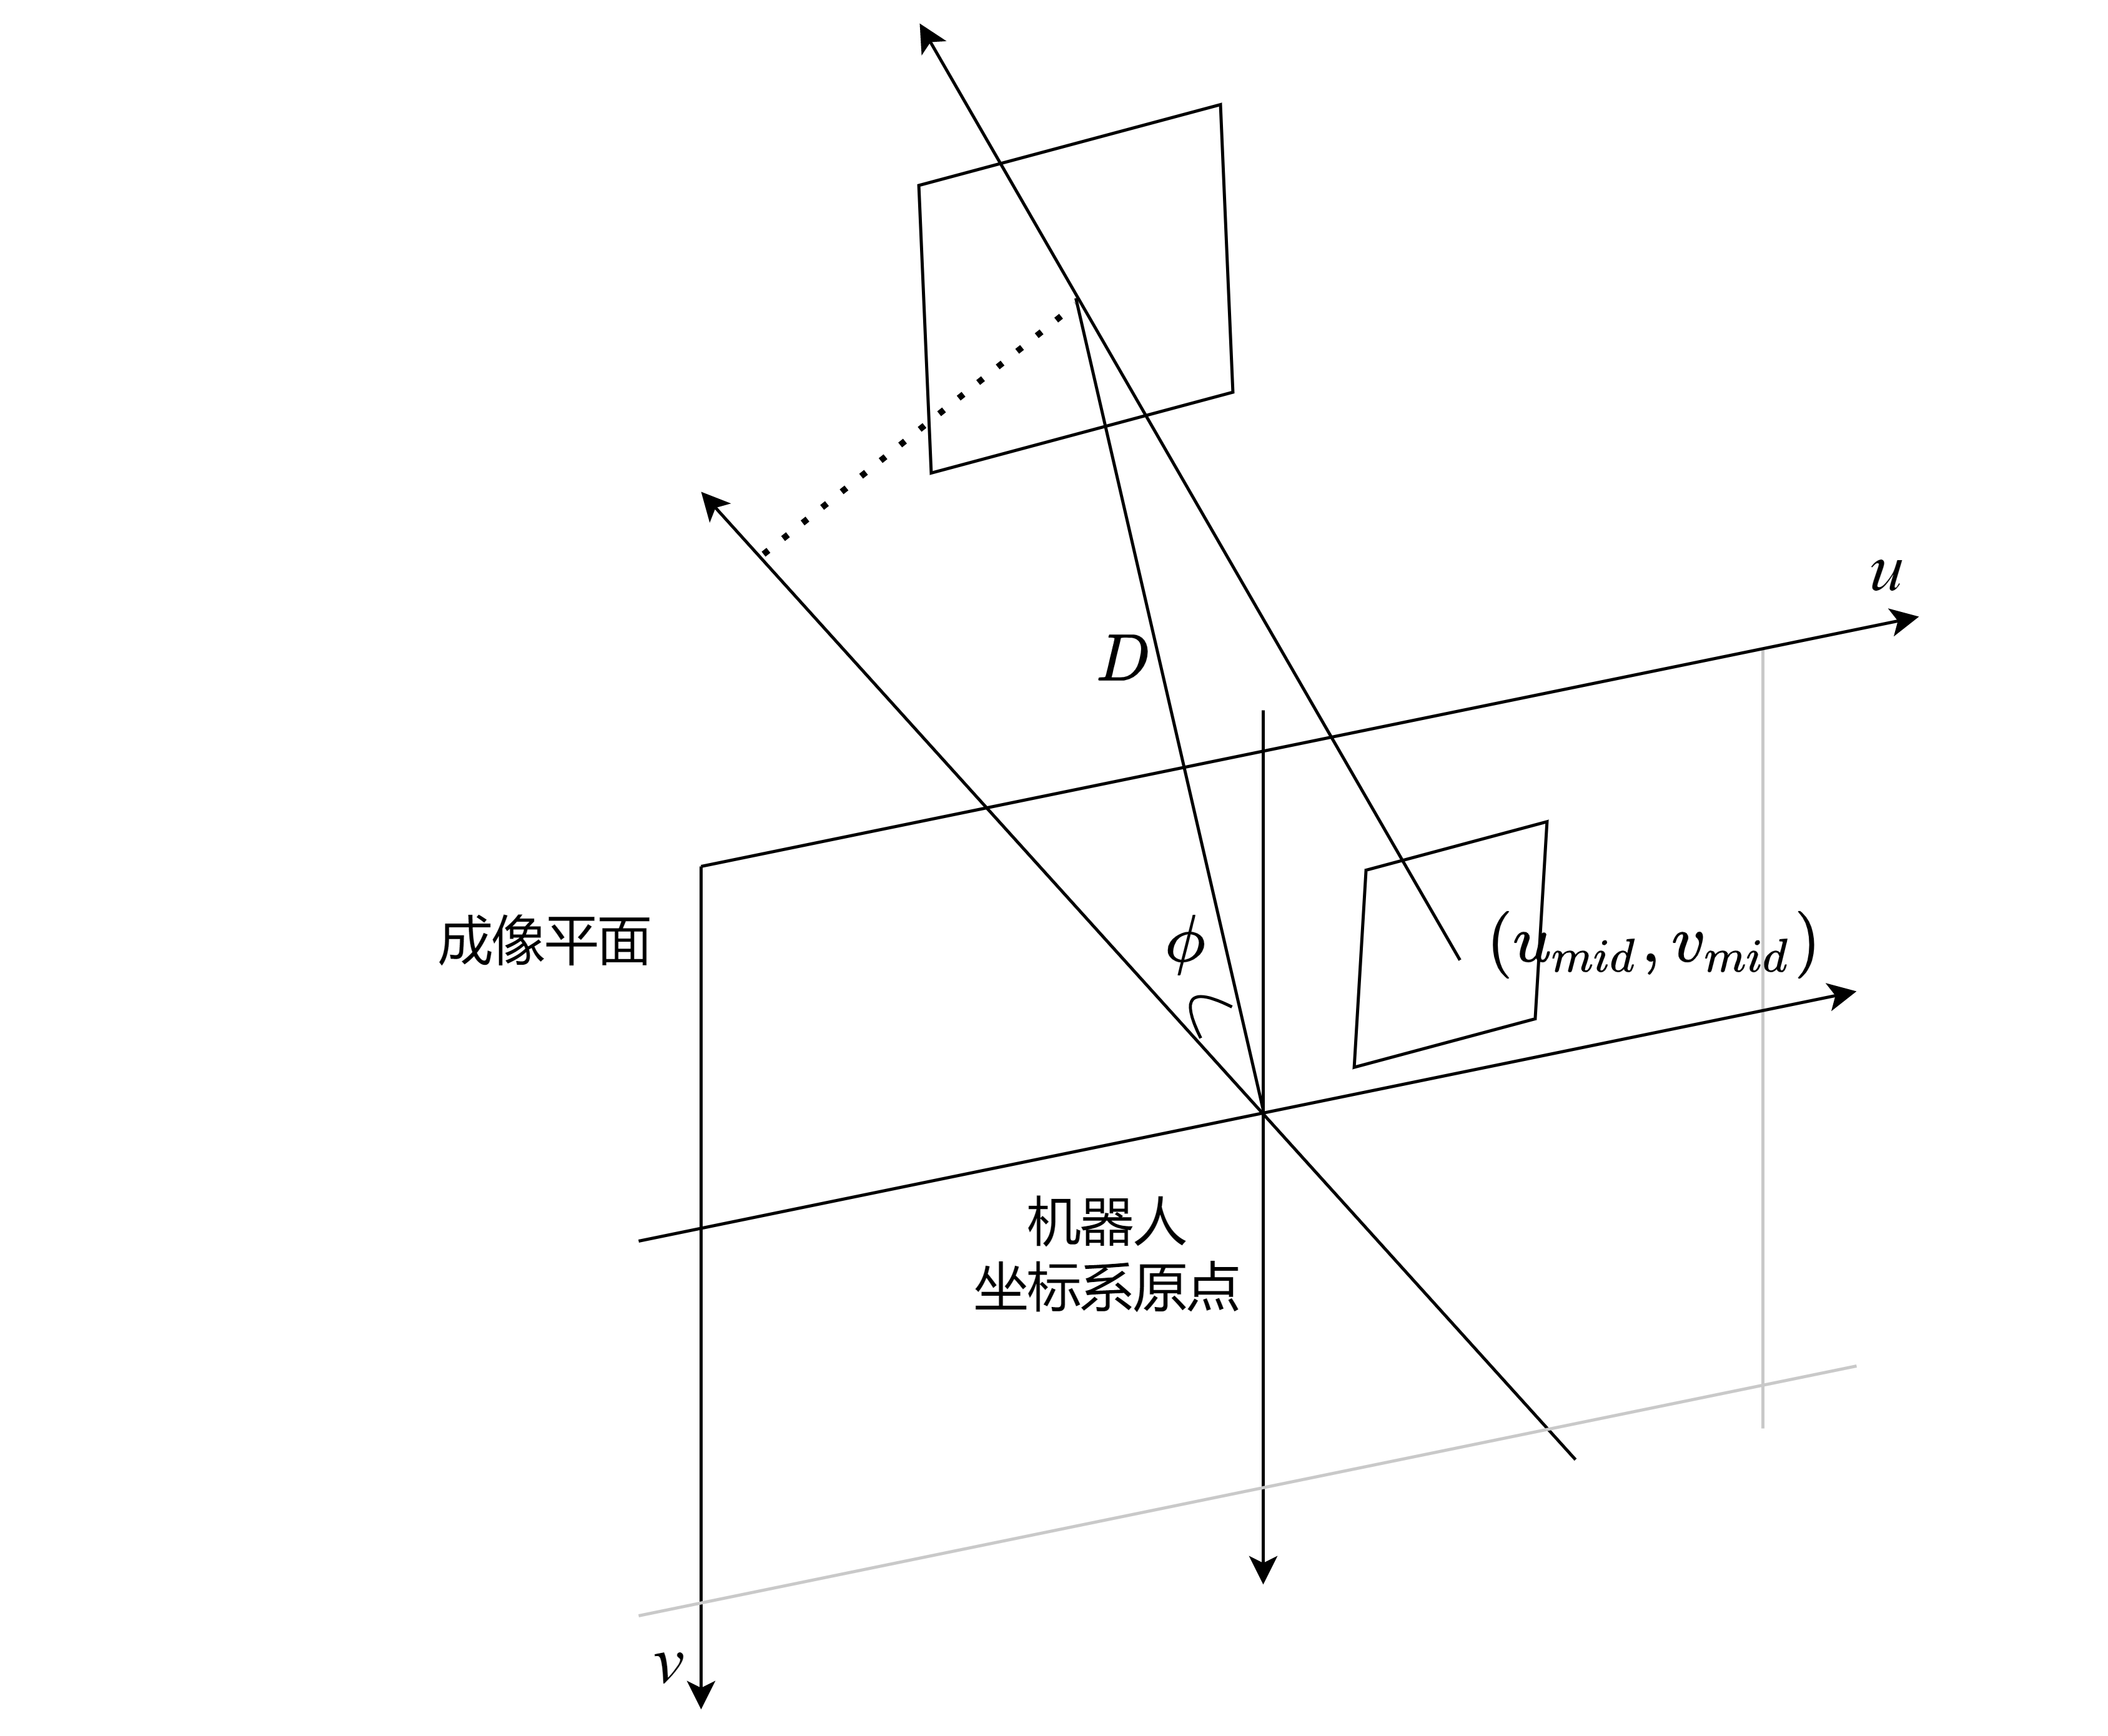
\includegraphics[scale=0.12]{Fig/目标坐标..png}
    \caption{\label{target_pose}根据平面成像与点云数据求目标位姿}
\end{figure}
最后,通过ROS框架中tf话题所提供的数据和四元组转欧拉角方法即可将机器人坐标系下的目标位姿转换成地图坐标系下的目标位姿,发布导航即可完成完整的目标物体导航任务。需要注意的是,在实验的过程中我们发现当目标物处于桌子上等不可达的位置时,移动机器人将根据AMCL规划出的路径移动到环境的边界处,这通常与环境中离目标最近的导航点不一致,因此我们在发布最后的导航点时会先检查该点是否可达,当其不可达时图像点云融合模块将输出环境中与最终目标导航点相距最近的可达点作为替代。
具体的仿真环境、现实环境和消融实验实验结果见第五章。





\section{本章小结}
本章提出了一种局部路径规划方法,该方法由特征提取模块、特征融合模块、运动模块和图像点云融合模块构成。首先根据指令中目标物体的名称,通过特征融合、特征提取网络模型输出的离散动作,依靠运动节点在局部环境中进行自主探索,同时利用视觉图像信息识别出目标物体,在视觉观察中定位目标物体后再由图像点云融合算法计算获得目标的精确位姿,转换坐标系后发布导航任务完成局部环境目标物体导航。
